\documentclass[11pt]{article}

\usepackage{array}
\usepackage{amsmath}
\usepackage{booktabs}
\usepackage{caption}
\usepackage{dirtree}
\usepackage{fancyhdr}
\usepackage[a4paper, margin=1in]{geometry}
\usepackage{hyperref}
\usepackage[newfloat]{minted}
\usepackage{xcolor}
\usepackage{subcaption}
\usepackage{listings,cleveref}
\usepackage{newfloat} % https://tex.stackexchange.com/questions/95631/defining-a-new-type-of-floating-environment 2024-10-14
\usepackage{multimedia}
\usepackage[normalem]{ulem}
\usepackage[edges]{forest}
\usepackage[export]{adjustbox}
\usepackage{wrapfig}
\usepackage{tabularx}
\usepackage{graphics}
\usepackage{tikz}
\usepackage{pgf-umlcd}
\usepackage{ifthen}
\usepackage{xstring}
\usepackage{calc}
\usepackage{pgfopts}
% \usepackage{tikz-uml}
\usepackage{siunitx}
\usetikzlibrary{shapes.geometric, arrows}
\usetikzlibrary{arrows.meta} % for the hierarchy diagrams i think
\useunder{\uline}{\ul}{}
\renewcommand{\arraystretch}{1.2}

\definecolor{LightGray}{gray}{0.9}
\newcommand{\ra}[1]{\renewcommand{\arraystretch}{#1}}
% \textwidth = 415.37 pt

\renewcommand{\lstlistlistingname}{Code fragments}

\renewcommand{\umlfillcolor}{white}
\renewcommand{\umldrawcolor}{black}

% Types of floats: 
%   FIG     - Figure or Image file
%   PC      - Pseudocode snippet
%   SC      - Sourcecode snippet
%   TBL     - Table
%   FLOW    - Flowchart
%   FOR     - Forest
%   DIR     - Directory Tree

% for labels use this convention: 
% {sensible_identifier}_{type}{numbering(if necessary)}_{cycle/section_name}

\DeclareFloatingEnvironment[fileext=frm,placement={!ht},name=Code]{code}

% ps, fig, flow, for, dir is declared in a figure
% sc is declared in a listing
% tbl is declared in a table



% https://perso.ensta-paris.fr/%7Ekielbasi/tikzuml/var/files/doc/tikzumlmanual.pdf
% 2024-10-16 Class Diagrams

% Sections should have a linebreak above and below, except when going from a lower level to 
% a higher level in which case there should be two above the higher level.

% \pagebreak should have a line break above and below.

\setlength{\parindent}{0pt}


% Defining tikz styles for the flowcharts
\tikzstyle{startstop} = [rectangle, rounded corners, minimum width=3cm, minimum height=1cm,text centered, draw=black, ]
\tikzstyle{io} = [trapezium, trapezium left angle=70, trapezium right angle=110, minimum width=3cm, minimum height=1cm, text centered, draw=black,]
\tikzstyle{process} = [rectangle, minimum width=3cm, minimum height=1cm, text centered, draw=black,]
\tikzstyle{decision} = [diamond, minimum width=3cm, minimum height=1cm, text centered, draw=black, ]
\tikzset{%
    subprocess/.style = {rectangle, draw=black, fill=orange!30,
                         minimum width=3cm, minimum height=1cm, inner xsep=3mm,
                         text width =\pgfkeysvalueof{/pgf/minimum width}-2*\pgfkeysvalueof{/pgf/inner xsep},
                         align=flush center,
                         path picture={\draw 
        ([xshift =2mm] \ppbb.north west) -- ([xshift= 2mm] \ppbb.south west)
        ([xshift=-2mm] \ppbb.north east) -- ([xshift=-2mm] \ppbb.south east);
                                      },% end of path picture
                        }
}

\tikzstyle{arrow} = [thick,->,>=stealth]
\tikzstyle{darrow} = [dashed,->,>=stealth]


% These are for the directory trees which are pretty 
\definecolor{folderbg}{RGB}{124,166,198}
\definecolor{folderborder}{RGB}{110,144,169}
\newlength\Size
\setlength\Size{4pt}
\tikzset{%
    folder/.pic={%
        \filldraw [draw=folderborder, top color=folderbg!50, bottom color=folderbg] (-1.05*\Size,0.2\Size+5pt) rectangle ++(.75*\Size,-0.2\Size-5pt);
        \filldraw [draw=folderborder, top color=folderbg!50, bottom color=folderbg] (-1.15*\Size,-\Size) rectangle (1.15*\Size,\Size);
    },
    file/.pic={%
        \filldraw [draw=folderborder, top color=folderbg!5, bottom color=folderbg!10] (-\Size,.4*\Size+5pt) coordinate (a) |- (\Size,-1.2*\Size) coordinate (b) -- ++(0,1.6*\Size) coordinate (c) -- ++(-5pt,5pt) coordinate (d) -- cycle (d) |- (c) ;
    },
}

\forestset{%
    declare autowrapped toks={pic me}{},
    declare boolean register={pic root},
    pic root=0,
    pic dir tree/.style={%
        for tree={%
            folder,
            font=\ttfamily,
            grow'=0,
            directory,
            fit=band
        },
        before typesetting nodes={%
            for tree={%
                edge label+/.option={pic me},
            },
            if pic root={
                tikz+={
                    \pic at ([xshift=\Size].west) {folder};
                },
                align={l}
            }{},
        },
    },
    pic me set/.code n args=2{%
        \forestset{%
            #1/.style={%
                inner xsep=2\Size,
                pic me={pic {#2}},
            }
        }
    },
    pic me set={directory}{folder},
    pic me set={file}{file},
}


\begin{document}
    \pagestyle{fancy}
    \setlength{\headheight}{13.6pt}

    % Title page
    \begin{titlepage}
        \begin{center}
            \vspace*{1cm}
            \Huge
            \textbf{Computer Science NEA 2025} \\
            \vspace*{2cm}
            \LARGE
            \textbf{Nathan Tatkowski}

            \vfill
            \includegraphics*[width=0.4\textwidth]{figures/igsLogo.jpg} \\
            \Large
            Invicta Grammar School \\
            Centre Number: 61721 \\
            Candidate Number: 8324
        \end{center}
    \end{titlepage}

    \tableofcontents

    \newpage
    \listoffigures

    \newpage
    \listoftables

    \newpage
    \lstlistoflistings

    \pagebreak

    \fancyhead[L]{Nathan Tatkowski}


    \section{Analysis}

        \subsection{Problem Identification}
            Often times in physics, complex circuit diagrams have to be drawn and understood, and the opportunity to actually build them is not always available. A solution that could handle custom circuits as well as model and log different attributes quickly, accurately, and efficiently in order to help with building intuition in regard to how complex electrical systems function would be a useful tool that could help solve this issue.

            As I would like to do Mathematics at university, I have decided to do my writeup for my NEA in LaTeX in order to gain experience. This has added a lot of complexity, as I am relatively new to using LaTeX, especially regarding formatting my writeup to be readable as well as easy to follow.

        \subsection{Identification of why this problem is solvable by computational methods}
            The key requirements stated above (accuracy, haste, and clarity) lend themselves very well to using computational methods. Computers are able to make calculations orders of magnitude faster than by hand or by analogue machine, and to a virtually arbitrary degree of accuracy. Many modern central processing units (CPUs) are also able capable of making use of concurrent processing, further increasing the advantage that a computer would have over a human. Graphical processing units (GPUs) are specifically designed for parallel processing, making them especially useful for graphics, which would allow for high quality renders for the user to be able to see. Any data that you would need to consider can be displayed in a clear and user-friendly fashion, making it highly customisable to fit the individual person's needs and for many attributes to be studied at the same time.

        \subsection{Description of the Current System}
            Without using computer simulations, the usual process is to produce a handful of equations by hand that would model the attributes of an object, for example the path it takes in three-dimensional space. This has the benefit of giving exact values and equations that are very useful when trying to understand the underlying reasons for an event happening. For example when considering a pendulum, it is clear from the equation $$ T = 2 \pi \sqrt{\frac{L}{g}} $$ that the period of the pendulum $T$ does not depend on the mass of the object doing the swinging. However, when running computer simulations, such relationships may not be as obvious, and as computers aren't able to analytically solve problems (i.e. through the use of rigorous mathematics), this is a drawback that I will have to consider. A computer model of a circuit can only be so accurate, as there aren't enough resources or time in order to model every single electron, proton, and neutron and all the intricate interactions they have with each other in real time.
            

        \pagebreak

        \subsection{Identification of Stakeholders}
            After considering the problem I identified the following groups that could use a solution to this problem, as well as having useful insight on how a program like this should function.


            % Identified Groups
            \begin{itemize}
                \item \textbf{University Students} often have to deal with complex systems and a way of visualising them would be very beneficial. I have been able to contact a student at the University of Aberdeen doing a masters in electrical and mechanical engineering. Their name is Hugo, and they are 21-years-old.
                \item \textbf{A-Level Students}, specifically students taking physics,  would be able to greatly further their understanding of core concepts and be able to explore new ideas on their own. I have been able to communicate with Daniel, a year 12 physics student, about being a stakeholder for this project.
                \item \textbf{Teachers} of A-Level and below could make great use of simulation software in order to make learning much easier with models and demonstrations that are clear and easy to understand. I have been able to contact Mr Waters about being a stakeholder for this project, who teaches physics at Invicta Grammar School.
            \end{itemize}
            
        \subsection{Identification of User Needs and Acceptable Limitations}
            Summary of key takeaways from interviews:
            \begin{itemize}
                \item My stakeholders are people who generally enjoy doing physics and find it enjoyable, although they all acknowledge how much work it can be. As such, decreasing workload without completely eliminating need for human input would be important, as that would make it less enjoyable.
                \item People struggle with abstract concepts, and a common topic seems to be electricity and electricals systems, as well as visualising some key concepts in physics such as waves. Considering a way to visualise circuits and the physics going on in those would be useful all of my stakeholders.
                \item People find graphs very useful in visualisation and aiding intuition. Some sort of real-time graphing of attributes could be something useful to consider in the final product.
                \item All my stakeholders are competent in using simulation software, or don't mind spending time to learn how to use one properly. This would mean that accuracy and functionality could be prioritised over general user experience if necessary. 
            \end{itemize}

        \subsection{Existing Solutions}

            \subsubsection{Analytic Methods}
                Analytic methods are very common as they require little cost or set-up and their effectiveness only depends on how well you understand the physics that you are doing. Since my stakeholders enjoy doing physics and are also quite good at it, they are all well versed in spending time going through calculations in order to achieve a set of mathematical equations that describe the system being modelled. 

                % fig:daniel_working
                % Daniel's Working FIG
                \begin{figure}[!ht]
                    \centering
                    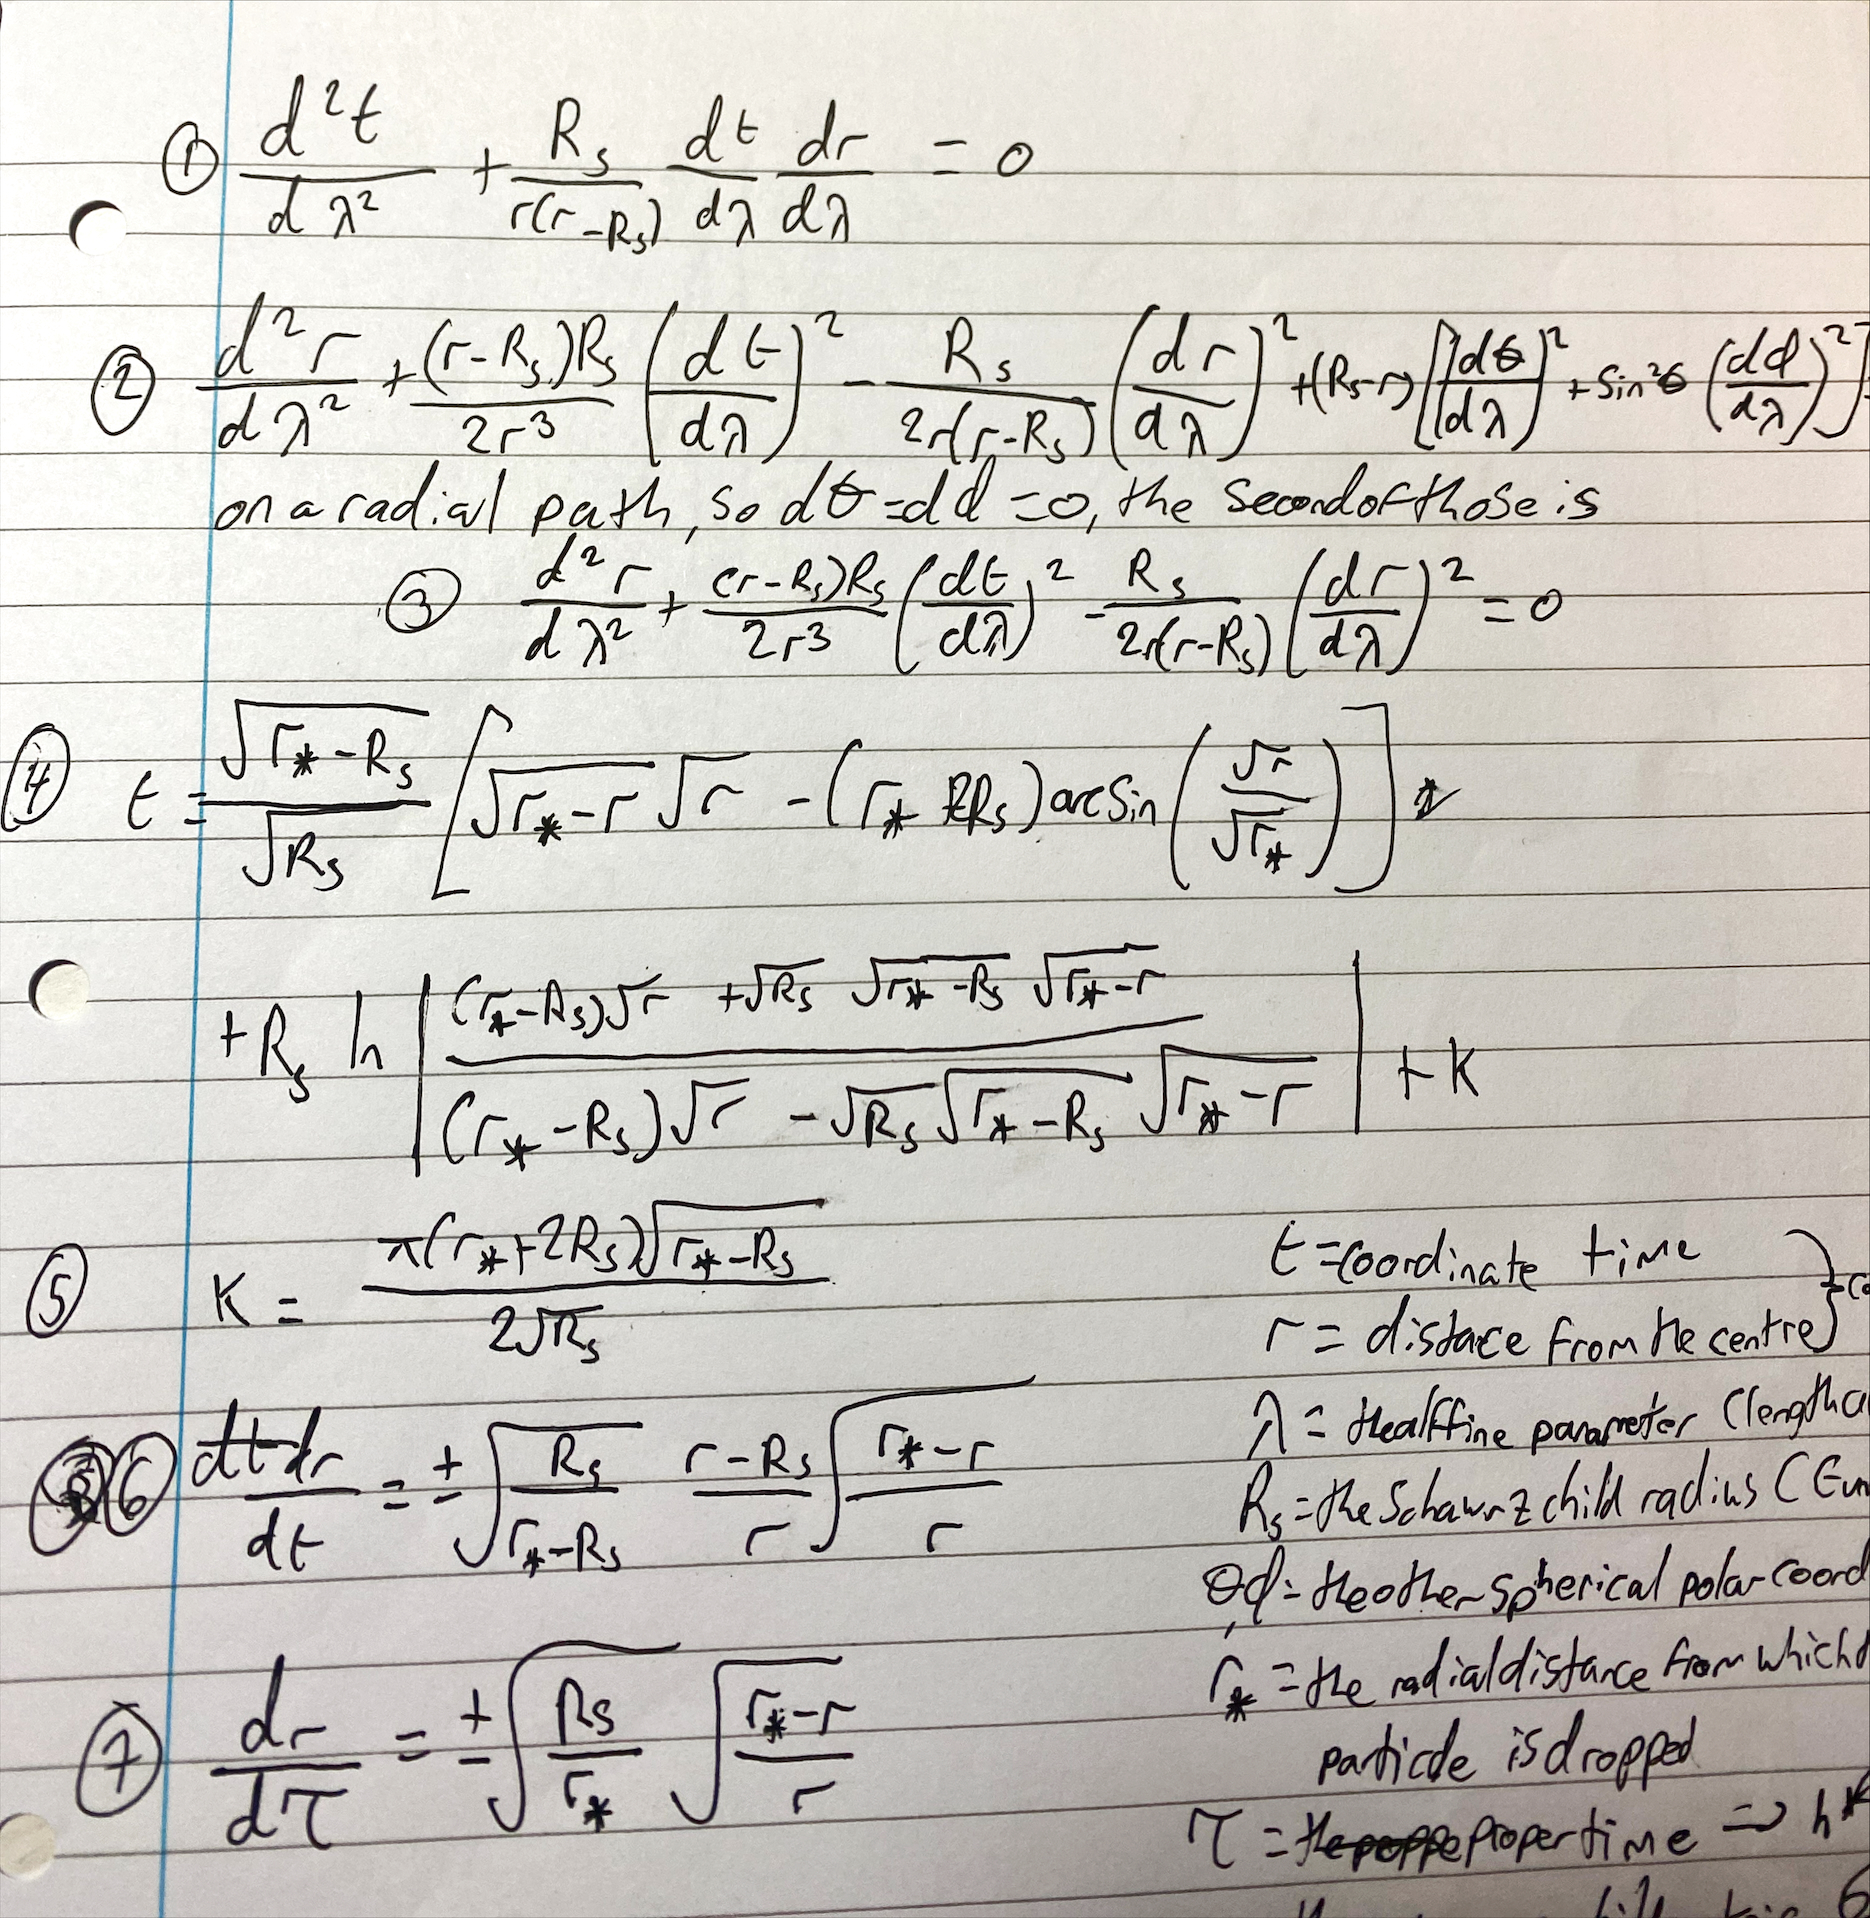
\includegraphics[width=0.25\textwidth]{figures/analysis/daniel_working.jpeg}
                    \caption{A sample of Daniel's working out}
                    \label{fig:daniel_working}
                \end{figure}

                \pagebreak

                \textbf{Advantages:}
                \begin{itemize}
                    \item Very versatile. Paper and pen allows for great customisation in the layout of the work including diagrams and annotations, which allows the user to be able to do things the way they want to do.
                    \item Cheap and easy to use. Little equipment is required and there isn't a need to install anything. 
                    \item Writing things physically on paper usually results in the writer being able to remember it easier, which would help in remembering things when learning. 
                    \item To get effective with analytic methods you require a lot of practice, which develops core skills like manipulation of various equations to achieve a desired result.
                    \item Ability to get exact answers and relationships between objects and attributes. Computers can only approximate exact answers and being able to see the equations of what is happening can greatly aid intuition when tackling future problems.
                    \item Doing hard work to get to a result is rewarding and relaxing. Offloading a lot of that work to a computer would reduce the enjoyment from this process.
                \end{itemize}

                \textbf{Disadvantages:}
                \begin{itemize}
                    \item Difficult to organise. You can't save paper notes in a way that is easily shareable and easy to organise on a computer (other than scanning them as PDF files which can take a lot of time and my clients find annoying). It may also be hard to stay consistent with formatting due to how versatile it is, as seen in \autoref{fig:daniel_working}.
                    \item Getting accurate graphs beyond simple sketches is difficult. Performing numerical methods by hand is very time-consuming which decreases the amount of time that can be spent on doing actual work. 
                    \item Scope of problems that can be approached is limited. Not all systems can be solved using analytic methods and sometimes numerical methods are necessary, depending on how simple or complex you choose to make your model.
                    \item Some problems are much harder to approach as the effectiveness of analytic methods is dependent on your ability to manipulate and work with equations, as well as general mathematical ability. Human's also make mistakes and are far less consistent than a computer at doing the same or similar calculations repeatedly.
                \end{itemize}

            \subsubsection{Desmos}

                % fig:desmos
                % Desmos FIG
                \begin{figure}[!ht]
                    \centering
                    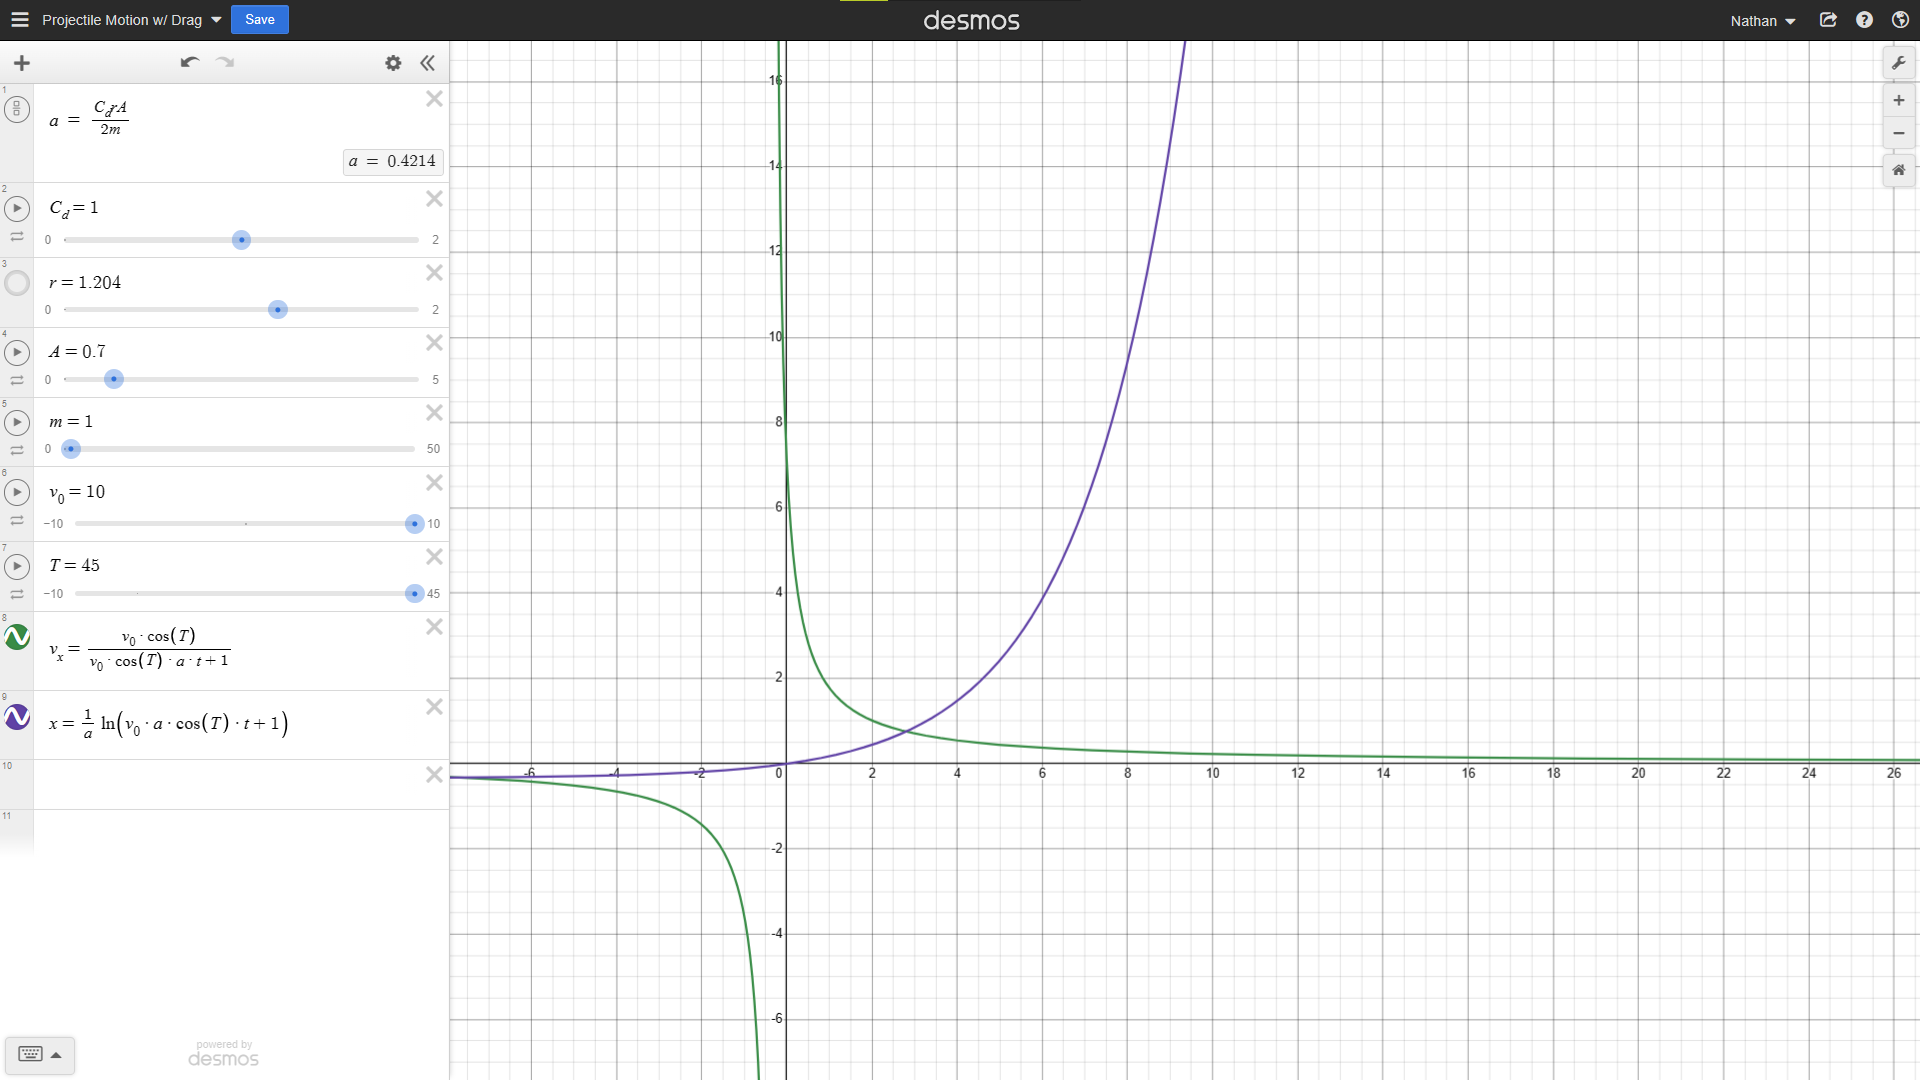
\includegraphics[width=.5\textwidth]{figures/analysis/desmos.png}
                    \caption{Desmos graphing software}
                    \label{fig:desmos}
                \end{figure}


                In \autoref{fig:desmos} below, Desmos has been used in order to see how attributes of an object change (specifically the $x$ position and velocity with respect to time of an object experiencing drag). Desmos is great in order to aid intuition and view general trends, however you still need to work through equations in order to have something to graph, and Desmos won't give exact values for solutions, but the final visualisations are still very useful. 

                The simplicity of Desmos allows it to be very versatile, but that also means its more of a jack-of-all-trades and master of none, so it wouldn't be very good for a more specialised application (like the ones being considered).

                % \newpage

                \textbf{Advantages:}
                \begin{itemize}
                    \item Desmos is a very versatile software which means that it can be used for a wide variety of problems. 
                    \item Free and easy to use. Desmos can be accessed by anyone with a computer or mobile device by going to \href{https://www.desmos.com/calculator}{their website}, or by downloading the mobile app.
                    \item Very customisable. Desmos allows for labels within the equation space, as well as changing the names of the labels on the axes. Which allows for some form of documentation within the graphs. The colours and line style are also changeable.
                    \item Easy to share and work on on multiple devices. After you make an account, you are able to save graphs that you've done and access them on whatever device you're signed in on. Graphs can also be shared with links once they're saved which allows for collaboration on projects.
                    \item As of quite recently, Desmos has released a beta for a 3D graphing mode, which is great for modelling some events happening in 3D, such as the trajectory of an object given some initial conditions.
                \end{itemize}


                \textbf{Disadvantages:}
                \begin{itemize}
                    \item The versatility of Desmos means that in the case of a more specialised system with specific needs, it would be more beneficial to create custom software for that specific system. However, Desmos still manages to cover a wide variety of problems, just not in a lot of depth.
                    \item The accuracy of Desmos is not very customisable, usually giving answers to two or three decimal places, and it is only able to give exact answers in some circumstances (values are usually given in terms of $\pi$ when working with trigonometric functions).
                    \item Circuits diagrams often end up messy and obviously not functional as they are on a piece of paper.
                \end{itemize}


            % do another one later
            
            \subsubsection{Online Circuit Builder}
                I searched for some online JavaScript based circuit builders and I found this \href{https://www.falstad.com/circuit/}{Circuit Simulator Applet}. Although none of my clients have used this before, and I don't personally have a lot of experience with it, I can see that there are a lot of good features in this solution. The use of circuit symbols instead of renders of components allows students to familiarise themselves with them, as when actually drawing out circuit diagrams that's what they would use. Furthermore, as circuits get more and more complex and components get smaller, it may not even be practical or useful to look at a real life version of the circuit. 

                % fig:circuit_builder_ss1
                % Circuit Builder SS FIG
                \begin{figure}[!ht]
                    \centering
                    \includegraphics[width=.5\textwidth]{figures/analysis/circuit_builder_1.png}
                    \caption{A simple circuit made on the circuit builder}
                    \label{fig:circuit_builder_ss1}
                \end{figure}


                % fig:circuit_builder_ss2
                % Circuit Builder graphs screenshot
                \begin{figure}[!ht]
                    \centering
                    \includegraphics[width=.5\textwidth]{figures/analysis/circuit_builder_graphs.png}
                    \caption{Graphs of attributes changing with respect to time and each other}
                    \label{fig:circuit_builder_ss2}
                \end{figure}


                \textbf{Advantages:}
                \begin{itemize}
                    \item The use of standard circuit symbols, which are 2D and quite simple shapes, instead of renders or images of actual components makes the program more efficient and increases performance, as no advanced rendering is necessary. 
                    \item Charge flow indicators in the form of yellow circles that represent electrons help visualise the flow of charge around a circuit for students. 
                    \item Including colour indicators do distinguish between places with negative and positive potential difference adds another level of interaction for the user, and this is something that could be quite hard to visualise and notice even with a real life version of the circuit available.
                    \item The simulation can be freely paused and unpaused in order to be able to see how a circuit appears at a specific point in time, which would be difficult with a real life version. 
                    \item The ability to plot real time graphs akin to an oscilloscope is as useful as having a real life oscilloscope, which is great when used to see how attributes change with respect to time and each other. See \autoref{fig:circuit_builder_ss2}.
                    \item The ability to export and import circuit arrangements is very useful as it allows for easier collaboration.
                \end{itemize}


                \textbf{Disadvantages:}
                \begin{itemize}
                    \item Although it contains a myriad of different components and pre-made circuits, some "features" are missing. For example, you can't set the internal resistance of a cell, and you also can't choose custom wires where you can alter the resistivity and length more precisely, which would make the simulation more accurate.
                    \item I found the system for placing new components in to be quite clunky and frustrating to get used to. Drawing the components is a good system, but the way it was implemented felt annoying to place in new components, it felt like you had to already know where you want to place components beforehand, which limits the freedom the user has to experiment with new arrangements. 
                \end{itemize}


        \subsection{Success Criteria of the Proposed System}
            See \autoref{tbl:essential_succ_crit} for a table of essential success criteria for the system. 


            See \autoref{tbl:optional_succ_crit} for a table of optional criteria for the solution, that would still benefit the users but aren't essential for it to be deemed functional and are mostly quality of life features.
        
        
        % \subsection{Data Source(s)}
        % \subsection{Volumetrics - Data Volumes}
        % \subsection{Analysis Data Dictionary}
        % \subsection{Data Flow Diagrams for Existing and Proposed System}

        \subsection{Justification of Chosen Solution}
            My proposed solution is to create a piece of software that functions as a electrical circuit builder allowing the user to place different components on a main board and then connect them using wires. Then the software would simulate what is happening at each component as well as allow those attributes to be viewed and logged by the user within the software. Circuits wouldn't be able to be edited while they are being simulated, as the two modes would be completely separate from each other.

            This solution would be very good as it would allow for a concept that a lot of students struggle with to be visualised. A lot of students do not have access to circuit components at home, and so trying to study circuits independently can be very challenging for some. A much larger proportion of students own a computer with a mouse and keyboard at their home, so a piece of software would be more accessible to most if not all students. Also, as education shifts more and more into digital, a way of collaborating on circuits through the internet (with just being able to send an exported file to another person) greatly aids student understanding and ability to learn.

        \subsection{Hardware and Software}
            The system will only require a computer with a working mouse and display to work properly, but the functionality for keyboard shortcuts is a possibility in the future. Regarding software, only the actual program is would be necessary, and distributing it to the end user would be a trivial task.

        \subsection{Limitations}
            I only have experience with GUI elements while using Python, however the complexity and amount of processing needed for the project may exceed the capabilities of Python. As such careful consideration into how features are implemented would have to be taken as I need the program to be as efficient as possible. 

        % \subsection{Entity-Relationship Models}
        % \subsection{Identification of Objects and Object Analysis Diagrams}


    \section{Overall System Design}
            I decided to split the system into three sections: project, simulating, building. Within the software, the user will initialise a "project" in a directory. The program will frequently refer to a "source directory", which will be the user's program files by default. This source directory will be configurable by the user, but there is no guarantee that the user changing things on their own won't break some of the functionality.

            % Overall Hierarchy Diagram FRST
            % \begin{center}
            %     \footnotesize
            %     \begin{forest}
            %         for tree={
            %             align=center,
            %             font=\sffamily,
            %         edge+={thick, -{Stealth[]}},
            %         l sep'+=10pt,
            %         fork sep'=10pt,
            %         },
            %         forked edges,
            %         if level=0{
            %             inner xsep=0pt,
            %             tikz={\draw [thick] (.children first) -- (.children last);}
            %             }{},
            %             [Circuit Builder
            %                 [Project/File Management
            %                     [Initialising
            %                         [Choose to\\make new or\\open file
            %                             [Importing\\all data and\\rendering]
            %                             [Initialising\\necessary files]
            %                         ]
            %                         [Choose working\\directory]
            %                     ]
            %                     [Exporting
            %                         [Data]
            %                         [Project/Circuit\\arrangement]
            %                     ]
            %                 ]
            %                 [Simulating
            %                     [Updating\\attributes of\\components
            %                         [Rendering\\updates]
            %                         [Storing data]
            %                     ]
            %                     [Rendering\\graphs]
            %                 ]
            %                 [Building
            %                     [Placing\\components
            %                         [Choosing\\component]
            %                         [Choosing\\location]
            %                     ]
            %                     [Editing\\attrib[utes
            %                         [Menu\\interactions]
            %                     ]
            %                 ]
            %             ]
            %         \end{forest}
            % \end{center}

            Each cycle will be taken on individually. I had to get rid of the overall hierarchy diagram because it wouldn't compile for some reason. (I will add it back later)
            
    \section{Cycle 1: Installation}
        Below is the hierarchy diagram for this cycle. Note that here "program" is used to refer to the entire program, and not just the installer covered in this cycle.

        % for:hierarchy_diagram_c1
        % Cycle 1 Hierarchy diagram
        \begin{figure}[!ht]
            \centering
            \footnotesize
            \begin{forest}
                for tree={
                    align=center,
                    font=\sffamily,
                edge+={thick, -{Stealth[]}},
                l sep'+=10pt,
                fork sep'=10pt,
                },
                forked edges,
                if level=0{
                    inner xsep=0pt,
                    tikz={\draw [thick] (.children first) -- (.children last);}
                    }{},
                    [Installation
                        [File management
                            [Hosting files]
                            [Updating files]
                        ]
                        [Installer
                            [Checking\\permissions
                                [Admin\\permissions]
                                [Directory\\validation]
                            ]
                            [Program\\configuration]
                            [Ease of use
                                [Add desktop\\shortcut]
                                [Uninstaller\\program]
                            ]
                        ]
                    ]
            \end{forest}
            \caption{Cycle 1 hierarchy diagram.}
            \label{for:hierarchy_diagram_c1}
        \end{figure}

        \subsection{Brief Outline}
            In this cycle I will create a way to install the program onto the user's computer using Python. This will also include an uninstall program which will allow the user to safely uninstall the program if they wish to do so.

            \subsubsection{Success Criteria}
                See \autoref{tbl:succ_crit_c1}.
                
        \subsection{Design}
            % Need to do UI and testing here, as well as talk more about how this is going to be implemented

            \subsubsection{User Interface}
                User interface (UI) windows will be implemented as classes that then have individual elements such as buttons, entries, and labels implemented as attributes of the class that can be edited as needed. Buttons will call methods in the class as their functions, allowing them to refer to other UI elements in the same window easily. See \autoref{fig:install_gui_class_diagram_c1}.

                % fig:install_gui_class_diagram_c1
                % InstallGUI Class Diagram FIG
                \begin{figure}[!ht]
                    \centering
                    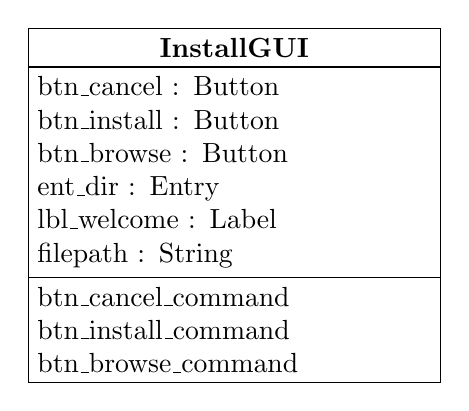
\begin{tikzpicture}
                        \begin{class}[text width=5cm]{InstallGUI}{0,0}
                            \attribute{btn\_cancel : Button}
                            \attribute{btn\_install : Button}
                            \attribute{btn\_browse : Button}
                            \attribute{ent\_dir : Entry}
                            \attribute{lbl\_welcome : Label}
                            \attribute{filepath : String}

                            \operation{btn\_cancel\_command}
                            \operation{btn\_install\_command}
                            \operation{btn\_browse\_command}
                        \end{class}
                    \end{tikzpicture}
                    \caption{InstallGUI class diagram}
                    \label{fig:install_gui_class_diagram_c1}
                \end{figure}

                In \autoref{fig:installer_gui_design_c1}, I have made a design for the graphical user interface of the installer part of this cycle. The user will be able to enter a directory on their computer in the white entry box, and then press the "Install" button which will then validate this input as well as download the files to the specified folder. The cancel button will quit the installer and no further processing will occur.

                % fig:installer_gui_design_c1
                % design for the installer gui 
                \begin{figure}[!ht]
                    \centering
                    \includegraphics[width=.5\textwidth]{figures/c1/design/installer_ui_design_mock.png}
                    \caption{UI Design}
                    \label{fig:installer_gui_design_c1}
                \end{figure}

                I chose the colours that I did for the button, as they were suggested to have high contrast with the black text on them, see \autoref{fig:high_contrast_ppt_pf_c1}. This aids accessibility, making it easier to see the text on each button. I believe that the text on each button also sufficiently describes their function, leaving no room for ambiguity, and the user can be confident in what each press will do. 

                % fig:high_contrast_ppt_pf_c1
                % Screenshot from ppt showing the "high-contrast only" toggle
                \begin{figure}[!ht]
                    \centering
                    \includegraphics[width=.5\textwidth]{figures/c1/design/high_contrast_ppt_pf.png}
                    \caption{High contrast colour suggestions by PowerPoint}
                    \label{fig:high_contrast_ppt_pf_c1}
                \end{figure}

                I want to be able to communicate to the user if an error occurs, with a special case for if the user inputs an invalid directory. I used text coloured red, which has negative connotations, that was also marked as high contrast, as well as messages that told the user that the input was invalid, or a message saying that an unknown error occurred, see \autoref{fig:installer_ui_design_errors_c1}. I don't think that other errors will need to be treated specially, as any that occur would be with the downloading process and out of the user's control.

                % fig:installer_ui_design_errors_c1
                %       fig:installer_ui_design_directory_error
                %       fig:installer_ui_design_other_error
                % Showing how errors will be handled by the UI
                \begin{figure}[!ht]
                    \begin{subfigure}{.5\textwidth}
                        \centering
                        \includegraphics[scale=0.5]{figures/c1/design/installer_ui_design_error_1.png}
                        \caption{Invalid directory error}
                        \label{fig:installer_ui_design_directory_error}
                    \end{subfigure}%
                    \begin{subfigure}{.5\textwidth}
                        \centering
                        \includegraphics[scale=0.5]{figures/c1/design/installer_ui_design_unknown_error.png}
                        \caption{Other unknown error}
                        \label{fig:installer_ui_design_other_error}
                    \end{subfigure}%
                    \caption{Design for communicating errors to the user}
                    \label{fig:installer_ui_design_errors_c1}
                \end{figure}

                In the event of a successful installation, I would also like to notify the user. To do this I used the word "Success!" coloured in high contrast green, which is a colour with positive connotations, shown in \autoref{fig:install_ui_successful_design_c1}.

                % fig:install_ui_successful_design_c1
                % installation ui after a successful installation
                \begin{figure}[!ht]
                    \centering
                    \includegraphics[width=.5\textwidth]{figures/c1/design/installer_ui_success.png}
                    \caption{Message after successful installation}
                    \label{fig:install_ui_successful_design_c1}
                \end{figure}


            \subsubsection{Data Structures}

                The user may not always have permissions to save into/export into the directory they have selected. When doing file management using for example the file explorer on Windows 10, the operating system will handle telling the user that they have invalid permissions. However, when attempting operations on files with invalid permissions through a programming language such as Python, the error will be raised in the program. Due to this I have included a \verb|permissions| variable that checks whether the program has permissions to write to a given directory to prevent this. See \autoref{tbl:data_structs_c1} for a table of data structures.

            \subsubsection{Algorithms}
                I decided to plan some of my key algorithms for this cycle, namely the algorithms responsible for exporting files, initialising a project, and installing the program.

                % flow:flowchart_design_c1
                % flowchart for exporting a project as a .zip file
                \begin{figure}[!ht]
                    \centering
                    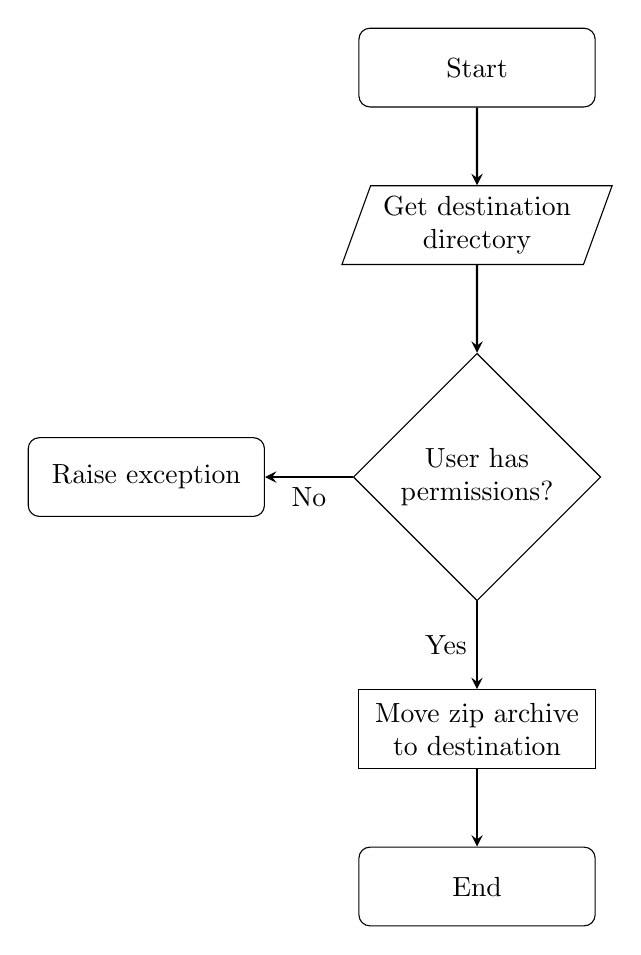
\begin{tikzpicture}[node distance=2cm]
                        \node (start) [startstop] {Start};
                        \node (in1) [io, below of=start, align=center] {Get destination\\directory};
                        \node (dec1) [decision, below of=in1, align=center, yshift=-1.2cm] {User has\\permissions?};
                        \node (exc1) [startstop, left of=dec1, xshift=-2.2cm] {Raise exception};
                        \node (pro1) [process, below of=dec1, align=center, yshift=-1.2cm] {Move zip archive\\to destination};
                        \node (end) [startstop, below of=pro1] {End};
                        \draw [arrow] (start) -- (in1);
                        \draw [arrow] (in1) -- (dec1);
                        \draw [arrow] (dec1) -- node[anchor=north] {No} (exc1);
                        \draw [arrow] (dec1) -- node[anchor=east] {Yes} (pro1);
                        \draw [arrow] (pro1) -- (end);
                    \end{tikzpicture}
                    \caption{Flowchart for exporting a project}
                    \label{flow:flowchart_design_c1}
                \end{figure}
                

                % pc:copy_to_folder_ps_c1
                % Initialise project PC
                \begin{figure}[!ht]
                    \begin{minted}[linenos]{python}
    import os
    source = "Source directory here"
    procedure init_files(target)
        if target.permissions == False:
            raise PermissionError
        files = os.listdir(source)
        for f in files:
            f.copy(target)
    endprocedure
                    \end{minted}
                    \caption{Pseudocode to copy initial project files to a folder}
                    \label{pc:copy_to_folder_ps_c1}
                \end{figure}


                The file running the procedure above will need to be in the same location as the folder it is copying from. To make the file easier to access, the program could make a shortcut to this file and add it to the desktop for the user.
                

                % pc:install_software_ps_c1
                % Install main program PC
                \begin{figure}[!ht]
                    \begin{minted}[linenos]{python}
    url = https://github.com/nathan-tat/cs_nea_2025/tree/main/code/software
    procedure install_software(target)
        if target.permissions == False:
            raise PermissionError
        
        download_from_github(url, target)
                    \end{minted}
                    \caption{Pseudocode to install the main program}
                    \label{pc:install_software_ps_c1}
                \end{figure}


                The installer will copy files from a GitHub repository, where all the files necessary for the program to run will be stored, into a folder specified by the user on the user's computer. This folder will then be referred to as \verb|source| (see \autoref{tbl:data_structs_c1}). This will hopefully be done through the use of an external library.

                Having multiple directories with the program downloaded or having broken installations could cause undesired outcomes. Due to this, I would like the user to use the "Close" button in order to terminate the program, and so I will include a check for this. A Python file will not necessarily terminate after a GUI window is closed, so it is still possible to do some processing after this. In the method written for the "Close" button, I will have a variable \verb|safety| set to \verb|True| and then check its value afterwards, alerting the user if this condition isn't met and possibly giving them some advice on how they can go forwards to guarantee that everything will work later on, see 

                % fig:installer_ui_design_unsafe_exit_c1
                % Little design for when the user doesn't exit the program safely. 
                \begin{figure}[!ht]
                    \centering
                    \includegraphics[width=.5\textwidth]{figures/c1/design/installer_ui_design_unsafe_exit.png}
                    \caption{Unsafe termination of the program alert}
                    \label{fig:installer_ui_design_unsafe_exit_c1}
                \end{figure}


        \subsection{Testing}

            See \autoref{tbl:test_data_before_c1} for the testing table for this cycle.


        \subsection{Implementation}
            % I neeed to ask if I'm doing a diary style implementation or the other one cause i have no clue
            % I find it easer to write some code, insert a screenshot of it working/not working, and then explaining why I did what I did/what I did to fix it

            % The installer will copy files from a specified repository on GitHub, which will store all the necessary files for the program to run, into a folder specified by the user, which will then be referred to by the program as the source folder. 


            % In \autoref{sc:if_name_main_c1}, there is code that is executed when the \verb|installer.py| file is run. This includes a check for whether the program is currently being run in administrator mode, shown in \autoref{sc:admin_checker}. This differs slightly from the design in \autoref{tbl:data_structs_c1}, where there was a variable defined to do the same thing. I found this implementation more readable and understandable, as using a function that returns a boolean value emphasises the fact that I want to check the permissions at a single moment in time. The code continues to start the UI so that the user can interact with the program. The code shown in \autoref{sc:admin_checker} is from StackOverflow. 
            % I am going to work on proper references at some point for this document


            When the Python interpreter reads a source file, it sets the variable \verb|__name__| to \verb|__main__| if the program is being run as the main program, or as the filename if the program is being imported.
            In order to avoid problems such as the installer being run unintentionally, I have decided to check the value of this variable to make certain that no code is executed in the case that the file is imported somewhere, see \autoref{sc:if_name_main_c1}.
            In this beginning if-statement, there is also a check for whether the program is being run using elevated privileges or not, using the function shown in \autoref{sc:admin_checker}. 
            This prevents the user from encountering errors when trying to install to a location that they don't have permission to.
            This part of the program is also when the GUI element is run from.


            % fig:installer_gui_ss1_c1
            % Installer GUI evidence FIG
            \begin{figure}[!ht]
                \centering
                \includegraphics[width=.5\textwidth]{figures/c1/implement/installer_gui_pf1.png}
                \caption{Installer in action}
                \label{fig:installer_gui_ss1_c1}
            \end{figure}


            While implementing the UI elements, I discovered that Tkinter, the Python library I decided to make use of for the UI, allowed for opening a pop-up dialogue in which the user could select a folder, as demonstrated in \autoref{fig:installer_gui_ss1_c1}.
            This avoided the need to validate the user's entry as well as the need for a user text input at all, since the user can only select directories that exist on their computer. 
            This also lead to the abandoning of a default install directory being entered for the user, which was initially introduced due to how awkward it would've been to input a directory.

            % fig:requirements-txt-c1
            % Requirements.txt file example
            \begin{figure}[!h]
                \centering
                \includegraphics[scale=.25]{figures/c1/implement/requirements_file.png}
                \caption{Requirements file}
                \label{fig:requirements-txt-c1}
            \end{figure}

            In the function tied to the Install button, see \autoref{sc:install_btn_sc_c1}, there are two functions called.
            The \verb|install_requirements| function installs all the necessary Python modules onto the users device referencing a text file that contains the names and version numbers of said modules, shown in \autoref{fig:requirements-txt-c1}. At first I had some trouble with this function as I wasn't calling the command with the correct flags, shown in \autoref{sc:install_reqs_fail1_c1}. 
            The \verb|download_from_github| function copies the files from a folder in a GitHub repository. 
            % The former of these makes sure that the user has all the necessary Python libraries installed on their device, so that the program can function properly. 
            % Originally, I was planning to completely make use of a Python library that would have allowed me to interact with the GitHub API, but I could not find one that would do that for me and work, instead I managed to find code that would do the same thing, which is shown in \autoref{sc:dl_from_github_stolen_c1}, courtesy of GitHub user \href{https://github.com/Nordgaren/Github-Folder-Downloader/tree/master}{Nordgaren}.


            % As previously mentioned, I want to use a function in order to make sure that the relevant Python libraries are installed, which is shown in \autoref{sc:install_reqs_fail1_c1}. 
            % When this function is called in the program, see \autoref{sc:install_btn_sc_c1} line 22, the \verb|REQ| constant from is always passed as the argument, which links to the \verb|requirements.txt| file in the GitHub repository. However, this feature doesn't work as intended, see \autoref{fig:install_reqs_fail_pf_c1}, so it is commented out in the current version.


            % fig:install_reqs_fail_pf_c1
            % cmd ss proof to show that it failed
            \begin{figure}[!ht]
                \centering
                \includegraphics[width=\textwidth]{figures/c1/implement/installer_req_fail1.png}
                \caption{Failure of install requirements function}
                \label{fig:install_reqs_fail_pf_c1}
            \end{figure}
            
            % fig:install-req-success
            % Success of install req function
            \begin{figure}[!h]
                \centering
                \includegraphics[width=\textwidth]{figures/c1/implement/install_req_success.png}
                \caption{Success of install requirements function}
                \label{fig:install-req-success}
            \end{figure}

            % I need to test it
            I then decided to implement the function in order to create a desktop shortcut, shown in \autoref{sc:create_shortcut_c1}. For this I also made the change of adding a checkbox to the user interface that would allow the user to decide whether or not to add a desktop shortcut, shown in \autoref{fig:checkbox-installer-gui}. 


            % fig:checkbox-installer-gui
            % Installer GUI with checkbox
            \begin{figure}[!h]
                \centering
                \includegraphics[scale=1]{figures/c1/implement/new_installer_gui.png}
                \caption{Installer GUI with checkbox}
                \label{fig:checkbox-installer-gui}
            \end{figure}

            Initially this feature didn't work, shown in \autoref{fig:shortcut-fail-c1}, but as after some tweaking to the file path, it worked, as shown in 

            % fig:shortcut-fail-c1
            % Shortcut failure
            \begin{figure}[!h]
                \centering
                \includegraphics[scale=.4]{figures/c1/implement/shortcut_make_fail_01.png}
                \caption{Shortcut not working}
                \label{fig:shortcut-fail-c1}
            \end{figure}

            % fig:
            % 
            \begin{figure}[!h]
                \centering
                \begin{subfigure}{.4\textwidth}
                    \centering
                    \includegraphics[width=.9\textwidth]{figures/c1/implement/shortcut-working-proof-01.png}
                    \caption{The code in the file}
                    \label{fig:sc-working-proof-1-c1}
                \end{subfigure}%
                \begin{subfigure}{.4\textwidth}
                    \centering
                    \includegraphics[width=.9\textwidth]{figures/c1/implement/shortcut-working-proof-03.png}
                    \caption{Code executed from the shortcut}
                    \label{fig:}
                \end{subfigure}%
                \caption{Proof of shortcut working}
            \end{figure}



        \subsection{Evaluation}
            In this cycle I have managed to reach all of my success criteria listed in \autoref{tbl:succ_crit_c1} except for being able to uninstall the program with the same file. I have decided to move the development of this function to a later cycle, after the main program has been developed as I need a clearer view of how the program file structure will look like. 

    \newpage
    \section{Cycle 2: Project Management}
        \subsection{Brief Outline}
            This cycle will cover initialising and opening "projects", which will be how the user will be able to save their work and access it at a later time. 
            
            % for:hierarchy_diagram_c2
            % Cycle 2 Hierarchy diagram
            \begin{figure}[!ht]
                \centering
                \footnotesize
                \begin{forest}
                    for tree={
                        align=center,
                        font=\sffamily,
                    edge+={thick, -{Stealth[]}},
                    l sep'+=10pt,
                    fork sep'=10pt,
                    },
                    forked edges,
                    if level=0{
                        inner xsep=0pt,
                        tikz={\draw [thick] (.children first) -- (.children last);}
                        }{},
                        [Project Management
                            [Opening projects
                                [Choosing working\\directory]
                                [Verifying files]
                            ]
                            [Initialising projects
                                [Initialising files]
                                [Choosing working\\directory
                                    [Naming projects]
                                ]
                            ]
                        ]
                \end{forest}
                \caption{Cycle 2 hierarchy diagram}
                \label{for:hierarchy_diagram_c2}
            \end{figure}

                
            \subsubsection{Success Criteria}
                See \autoref{tbl:succ_crit_c2}.


        \subsection{Design}
            % The general idea is that it will use one program (this is the same one that the installer creates a shortcut to).
            % From then the user will be able to choose whether to open a new or existing project
            % If an existing project then the user will navigate to the project file inside the project folder, select it, and then it will use that to open everything necessary
            % If a new project then the user will select the DIRECTORY where they want the project file to be in. They will also decide on a name. I might also decide to include a drop down menu to select some kind of "type" or something.

            The idea of this cycle is that it will use one program, which is the one that the installer creates a shortcut to, from which the user will be able to decide whether to open a new or existing project. If the user chooses the former, then they will be prompted to select the \textit{directory} in which they would like to initialise their project, and if the latter then they will be prompted to select the \textit{project file} for their project. 
            The user will initially start on one user interface screen and depending on their choice go to one of two other user interface screens.

            \subsubsection{Data Structures}
                
                A data structure that allows the user to select their most recent projects from a list will need to be designed, as a consequence of the user interface design shown in \autoref{fig:menu_1_design_c2}.
                This data structure will need to be First In First Out, similar to a queue, however I would like it to only hold a maximum of three items. 
                See \autoref{flow:queue_like_design} for details.

                % flow:queue_like_design
                % Design for the queue-like data structure
                \begin{figure}[!ht]
                    \centering
                    \begin{tikzpicture}[node distance=2cm]
                        \node (2) [process, align=center] {B};
                        \node (1) [process, left of=2,  align=center, xshift=-2.0cm] {A};
                        \node (3) [process, right of=2, align=center, xshift=2.0cm] {C};

                        \node (4) [process, below of=1, align=center, ] {A};
                        \node (5) [process, below of=2, align=center, ] {B};
                        \node (6) [process, below of=3, align=center, ] {C};
                        \node (7) [process, right of=6, align=center, xshift=2.0cm] {D (New item)};

                        \node (8) [process, below of=5, align=center, ] {B};
                        \node (9) [process, below of=6, align=center, ] {C};
                        \node (10) [process, below of=7, align=center, ] {D};

                        \draw [arrow] (2) -- (1);
                        \draw [arrow] (3) -- (2);
                        \draw [darrow] (5) -- (4);
                        \draw [arrow] (6) -- (5);
                        \draw [arrow] (7) -- (6);
                        \draw [arrow] (9) -- (8);
                        \draw [arrow] (10) -- (9);
                    \end{tikzpicture}
                    \caption{How the queue-like structure will operate. Arrows point to the next oldest item.}
                    \label{flow:queue_like_design}
                \end{figure}
                
                This structure will be implemented with the use of a "global" text file (in the sense that changes to the text file on a local scale are reflected for every project) that will store projects in order of being opened.
                
                % fig:file-q-class-diagram
                % FileQueue class diagram
                \begin{figure}[!ht]
                    \centering
                    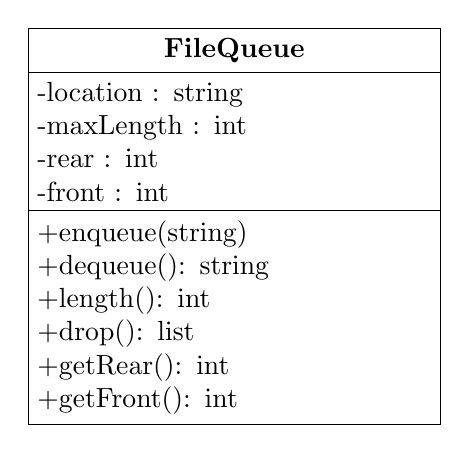
\begin{tikzpicture}
                        \begin{class}[text width=5cm]{FileQueue}{0,0}
                            \attribute{-location : string}
                            \attribute{-maxLength : int}
                            \attribute{-rear : int}
                            \attribute{-front : int}


                            \operation{+enqueue(string)}
                            \operation{+dequeue(): string}
                            \operation{+length(): int}
                            \operation{+drop(): list}

                            \operation{+getRear(): int}
                            \operation{+getFront(): int}
                        \end{class}
                    \end{tikzpicture}
                    \caption{FileQueue class diagram}
                    \label{fig:file-q-class-diagram}
                \end{figure}

                This class will allow me to easily access the FileQueue for the user's projects. 
                
                % dir:project_directory_tree_example_c2
                % Directory tree for an example project
                \begin{figure}[!ht]
                    \centering
                    \begin{forest}
                        pic dir tree,
                        pic root,
                        for tree={% folder icons by default; override using file for file icons
                            directory,
                        },
                        [project-name
                            [arrangements.json, file
                            ]
                            [config.json, file
                            ]
                        ]
                    \end{forest}
                    \caption{Directory tree example}
                    \label{dir:project_directory_tree_example_c2}
                \end{figure}

                % USed JSON cause it was easier
                % Didnt use SQL/database because i dont need them to be connected in any way and there is only a small amount of data involved

                
                Each directory that contains a project will include a configuration JSON file that will inform the main program on how to treat the project. I have decided to use JSON as it integrates nicely with Python (using the json module), as well as allowing me to create a template that each project can follow. 


                As shown in \autoref{ps:json_proj_config_example}, multiple properties regarding the project will be stored. Some of these will be set at the beginning and not changed again, such as \verb|directory|, and others are able to change even after the project's initial creation, in particular \verb|last_opened| will need to updated whenever the project is opened. Note that double backwards slashes are used for the \verb|directory| attribute, as a backwards slash is used as an escape character in the JSON file format.

                % ps:json_proj_config_example
                % Example for the JSON config file for a project
                \begin{figure}[!ht]
                    \begin{minted}[linenos]{json}
{
    "directory": "C:\\users\\...",
    "name": "this is a project name",
    "type": "project type",
    "created": "UNIX timestamp",
    "lastOpened": "UNIX timestamp"
}
                    \end{minted}
                    \caption{Configuration JSON file example}
                    \label{ps:json_proj_config_example}
                \end{figure}


                In \autoref{dir:project_directory_tree_example_c2}, I have designed the file structure for a single project. 
                The \verb|arrangements.json| file will hold how the components are arranged on the board. This is what the main program will use to run. 
                See \autoref{ps:json_proj_config_example} for the layout of \verb|config.json|.


                % fig:project-class-diagram-c2
                % Project class diagram
                \begin{figure}[!ht]
                    \centering
                    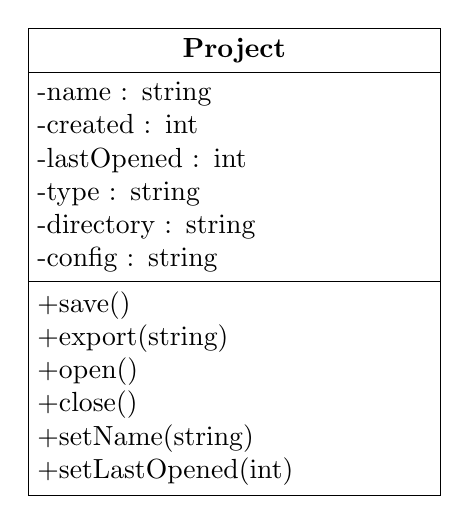
\begin{tikzpicture}
                        \begin{class}[text width=5cm]{Project}{0,0}
                            \attribute{-name : string}
                            \attribute{-created : int}
                            \attribute{-lastOpened : int}
                            \attribute{-type : string}
                            \attribute{-directory : string}
                            \attribute{-config : string}

                            \operation{+save()}
                            \operation{+export(string)}
                            \operation{+open()}
                            \operation{+close()}

                            \operation{+setName(string)}
                            \operation{+setLastOpened(int)}
                        \end{class}
                    \end{tikzpicture}
                    \caption{Project class diagram}
                    \label{fig:project-class-diagram-c2}
                \end{figure}

                I have again decided to make use of object-oriented programming this time in order to have a class for an instance of a running program, a class diagram of which is shown in \autoref{fig:project-class-diagram-c2}.

            \subsubsection{User Interface} 
                % Need to design 3 UI windows. 
                % One initial one that will then decide to go into one of the other two 

                % The initial one only needs two options, but something like a "recently viewed" might be nice.
                % It also will need a cancel option.

                % If user decides to open existing project, then need a browse directory button, as well as a confirm button. I don't think it needs anything more than that.
                % I think this could have a dropdown that could open a template 
                
                % If user decides to open new project, then need a "Name" entry, as well as a directory entry. Also confirm and cancel buttons. 

                There will be three user-interface menus covered in this section, one for where the user decides to open a new or existing project, and one each for actually selecting the project they want to open/create. 
                This was mainly inspired by the user-interface from Visual Studio 2022, see \autoref{fig:vs22_ui_ss_c2}, which shows a minimal design with only the necessary features shown.
                The layout is also very user-friendly, with large clear buttons shown as well as recently opened/viewed projects.

                % fig:vs22_ui_ss_c2
                % Screenshot from visual studio 22 that shows the UI for opening a project
                \begin{figure}[!ht]
                    \centering
                    \includegraphics[width=.5\textwidth]{figures/c2/design/vscode22.png}
                    \caption{Screenshot from Visual Studio 2022}
                    \label{fig:vs22_ui_ss_c2}
                \end{figure}

                With the colour-scheme, I have decided to stay consistent with my user interface from Cycle 1. The colours, borders, and fonts are the same. 
                I have decided to follow a similar layout to the one shown in \autoref{fig:vs22_ui_ss_c2}, but I chose to only have buttons for the three most recently viewed projects, as opposed to all of them sorted by date. 
                If the user has yet to open three projects, then the others would be greyed out and the user would not be able to click on them. 
                The justification for only showing three is that it could be difficult to implement an embedded window that allows the user to scroll through it independently of the rest of the window, and that the user will likely not not be working on more than three at a time. 

                % fig:menu_1_design_c2
                % first UI menu to show
                \begin{figure}[!ht]
                    \centering
                    \includegraphics[width=.5\textwidth]{figures/c2/design/ui1.png}
                    \caption{Design for first menu}
                    \label{fig:menu_1_design_c2}
                \end{figure}

                A change I have made in \autoref{fig:menu_2_design_c2} compared to \autoref{fig:menu_1_design_c2} is moving the "Cancel" button to the bottom left corner instead of keeping it in the bottom right corner. I decided this was better as it stayed consistent with the previous cycle, see \autoref{fig:installer_gui_design_c1}, and that that is how people tend to read (the order being top left, top right, bottom left, bottom right, according to \href{https://www.interaction-design.org/literature/article/visual-hierarchy-organizing-content-to-follow-natural-eye-movement-patterns}{the Interaction Design Foundation}). As part of my reflection from the first cycle, I have decided to include a "Browse" button, which will allow the user to select a directory using the familiar user interface of their operating system, as opposed to being forced to type in their directory manually. This is better as it increases usability. 

                % \clearpage
                % fig:menu_2_design_c2
                % design for opening a menu 
                \begin{figure}[!ht]
                    \centering
                    \includegraphics[width=.5\textwidth]{figures/c2/design/ui2_open_existing.png}
                    \caption{Design for opening an existing project}
                    \label{fig:menu_2_design_c2}
                \end{figure}

                % \newpage
                In \autoref{fig:init_new_proj_ui_design_c2}, I have designed the user interface for initialising a new project. The user will be allowed to select the name of the project and the directory in which the project is stored. I have also decided to include a dropdown selection box that would allow the user to select the "type" of project. At this time, I am not certain of what that exactly refers to. However, in the future I could use it for something. For example, the user being able to choose from a selection of pre-made circuits as a demonstration of the software.

                % fig:init_new_proj_ui_design_c2
                % design for the ui for initialising a new project
                \begin{figure}[!ht]
                    \centering
                    \includegraphics[width=.5\textwidth]{figures/c2/design/ui2_init_new_proj.png}
                    \caption{Design for initialising a new project}
                    \label{fig:init_new_proj_ui_design_c2}
                \end{figure}

                Following the menu from \autoref{fig:menu_2_design_c2} and \autoref{fig:init_new_proj_ui_design_c2}, the user will be taken to the main program, which will be taken on in a separate cycle.


            \subsubsection{Algorithms}
                % I'll need an algorithm for "opening" a project. i.e. passing off a directory as an argument to another function.
                % I'll need an algorithm to initiate a configuration file
                % I'll also need to think about how I will be able to lead from one UI element to another, something like this https://stackoverflow.com/questions/19473072/show-another-ui-file-on-button-click

                For this cycle I have decided to plan some key algorithms. These include algorithms to initiate a configuration file, opening a project, and updating the queue-like data structure.

                % pc:init_config_file_c2
                % Pseudocode to initiate the configuration file in a project folder from UI
                \begin{figure}[!h]
                    \begin{minted}[linenos]{python}
import json

def create_config_file():
    dictionary = {
        "directory": ent_directory.text,
        "project_name": ent_name.text,
        "type": drop_type.text,
        "created": UNIX(),
        "last_opened": UNIX()
    }

    with open("config.json") as file:
        json.dumps(dictionary, file)
                    \end{minted}
                    \caption{Pseudocode to initiate configuration file}
                    \label{pc:init_config_file_c2}
                \end{figure}


                % Opening a project

                % Updating Queue 

                \newpage

                % pc:fileq-length-method
                % PC for length of the file queue
                \begin{figure}[!h]
                    \begin{minted}[linenos]{python}
def length(self):
    return self.rear - self.front + 1
                    \end{minted}
                    \caption{Pseudocode to return the length of the FileQueue}
                    \label{pc:fileq-length-method}
                \end{figure}

                Note that in \autoref{fig:file-q-class-diagram} the \verb|length()| method is not a getter, as there is no length attribute defined in the class, which may be different to other implementations. For example in Python where \verb|len()| is an in-built function that takes in any iterable object, or in JavaScript where \verb|length| is an attribute. This method will mostly be used in order make some checks for the other functions in order to catch some edge cases. 

                % pc:enq-for-file-q
                % Code to enqueue to file queue
                \begin{figure}[!h]
                    \begin{minted}[linenos]{python}
def enqueue(self, project_id):
    # if the queue is full
    if self.length() == self.maxLength:
        self.front += 1

    self.rear += 1
        
    file = open(self.location)
    file.write(project_id)
    file.close()
                    \end{minted}
                    \caption{Pseudocode to add project to a FileQueue}
                    \label{pc:enq-for-file-q}
                \end{figure}

                In \autoref{pc:enq-for-file-q}, the amount of items in the queue is checked in order to make sure the pointers are changed properly. For example an edge case that could be considered is when an item is added to the FileQueue and there is no need to remove the oldest item as the FileQueue is not full, illustrated in \autoref{flow:fileq-not-full}.

                % flow:fileq-not-full
                % FileQueue when not full
                \begin{figure}[!h]
                    \centering
                    \begin{tikzpicture}[node distance=2cm]
                        \node (1) [process, align=center, ] {A};
                        \node (2) [process, right of=1, align=center, xshift=2.0cm] {B};

                        \node (3) [process, below of=1, align=center, ] {A};
                        \node (4) [process, below of=2, align=center, ] {B};
                        \node (5) [process, right of=4, align=center, xshift=2.0cm] {C};

                        \draw[arrow] (2) -- (1);

                        \draw[arrow] (4) -- (3);
                        \draw[arrow] (5) -- (4);

                    \end{tikzpicture}
                    \caption{Desired FileQueue behaviour when not at maxLength. C is added without A being removed.}
                    \label{flow:fileq-not-full}
                \end{figure}

                Essentially, the \verb|front| pointer is only incremented whenever the FileQueue is already at maximum capacity.

        \newpage
        \subsection{Testing}
            See \autoref{tbl:test-data-cycle2}.

        \subsection{Implementation}
            \subsubsection{CSV2LaTeX}
                In the middle of creating \autoref{tbl:test-data-cycle2}, I found it very tedious to type in the data manually straight into LaTeX code, which prompted me to consider other methods. 
                Since I find the user interface of Microsoft Excel quite easy to work with and well suited to manipulating tabular data, as well as CSV files easy to manipulate in Python, I wrote a Python script (including GUI) that would take in a CSV file and output a formatted table in LaTeX. 

                % pc:csv2latex-example-input-csv
                % Example input CSV file
                \begin{figure}[!h]
                    \begin{minted}[linenos]{text}
This,is,a,test
hello,world,foo,bar
1,2,3,4
words,words,words,words
                    \end{minted}
                    \caption{Example input CSV file. The top row includes the table headers.}
                    \label{pc:csv2latex-example-input-csv}
                \end{figure}


                % pc:csv2latex-example-output-latex
                % Example LaTeX table output
                \begin{figure}[!h]
                    \begin{minted}[linenos]{latex}
% tbl:example-for-nea
% Example table
\begin{table}[!h]
    \centering
    \begin{tabular}{@{}llll@{}} \toprule
        \textbf{This} & \textbf{is} & \textbf{a} & \textbf{test} \\ \midrule 
        hello & world & foo & bar \\ 
        1 & 2 & 3 & 4 \\ 
        words & words & words & words \\ 
        \bottomrule
    \end{tabular}
    \caption{This is what an example table looks like}
    \label{tbl:example-for-nea}
\end{table}
                    \end{minted}
                    \caption{Example LaTeX code output}
                    \label{pc:csv2latex-example-output-latex}
                \end{figure}


                % fig:rendered-csv2latex-table
                % Rendered LaTeX table
                \begin{figure}[!h]
                    \centering
                    \includegraphics[scale=.25]{figures/c2/implement/example-tbl.png}
                    \caption{The rendered LaTeX code}
                    \label{fig:rendered-csv2latex-table}
                \end{figure}

                First I wrote a function to work from a CSV file and write the LaTeX code from there, shown in \autoref{sc:csv2latex-func}. 
                It takes in the path to the CSV input file, the desired label, caption, and title, and whether or not the CSV file includes the table headers or not. Using that, I formatted the data from the CSV file by following LaTeX code I had previously written. 
                This function returns the LaTeX code as a string, not yet writing it to an output text file. 

                Working with just this function within a Python file would have been fine, however in order to account for maintainability, I tried to make it as easy as possible for people other than me to create new tables, taking into consideration that LaTeX is specialist knowledge. For example in the case where multiple people are working on the documentation, they should use the same table formatting in order to stay consistent. 
                This prompted me to develop a GUI front-end to the script. 

                I again decided to use a class for the main GUI element and implement button functionality as methods of the class, the constructor of the class (where labels, entries, and buttons are defined) are shown in \autoref{sc:csv2latex-gui-init-1}, \autoref{sc:csv2latex-gui-init-2}, and \autoref{sc:csv2latex-gui-init-3}. 
                I had also defined the \verb|input| and \verb|output| attributes, which are the input and output file paths respectively. 

                Inspired by the previous implementation in Cycle 1, a browse button was added, the method for which is shown in \autoref{sc:csv2latex-browse-method}. 
                This would allow the user to convert a CSV file from anywhere on the computer, allowing for the possibility of keeping a folder with a CSV file per table in the document which would make it easy to maintain them. 



                


                
        \subsubsection{FileQueue}
            I decided to implement the FileQueue first, as it was more standalone than the Project class and so better to do first. 

            \vspace{10pt}
            The constructor method for the FileQueue is shown in \autoref{sc:fileq-constructor}. The attributes have remained the same as in the design, shown in \autoref{fig:file-q-class-diagram}, \verb|__maxLength| and \verb|__location| are defined from the parameters, and \verb|rear| and \verb|front| are first defined as 0. 

            Since the items in the FileQueue are read from a source text file, it follows that the initial values for the front and rear pointers depend on the state of the source at the time of initialisation. This only affects the front pointer, as the rear pointer always points to the last item in the source. 

            % flow:fileq-front-ptr-init-bad
            % Showing how the front pointer gets initialised
            \begin{figure}[!h]
                \centering
                \begin{tikzpicture}[node distance=2cm]
                    \node (1) [process, align=center, ] {A (Non-existent)};
                    \node (2) [process, right of=1, align=center, xshift=2.0cm] {B};
                    \node (3) [process, right of=2, align=center, xshift=2.0cm] {C};
                    \node (4) [process, right of=3, align=center, xshift=2.0cm] {D};

                    \node at (0, -1.3) {-1};
                    \node at (4, -1.3) {0};
                    \node at (8, -1.3) {1};
                    \node at (12, -1.3) {2};

                    \node at (12, 1.3) {rear};
                    \node at (0, 1.5) {rear - maxLength + 1};
                    \node at (0, 1.1) {(Wrong)};

                    \draw[arrow] (4) -- (3);
                    \draw[arrow] (3) -- (2);
                    \draw[arrow] (2) -- (1);
                    \draw[dashed] (2,-1.5) -- (2,1.7);
                \end{tikzpicture}
                \caption{How the front pointer could be wrongly initialised}
                \label{flow:fileq-front-ptr-init-bad}
            \end{figure}

            \autoref{flow:fileq-front-ptr-init-bad} shows how the front pointer could be mistakenly initialised to a negative value if the source has not yet got maxLength items, which would cause unwanted behaviour later (in Python, accessing the $n$th index, where $n$ is negative, results in the $n$th to last item being returned, i.e. not raise an exception, which would make it hard to debug). Similar precautions were taken when implementing the enqueue method (the front pointer need not be decremented if the FileQueue has not reached maxLength).

            \vspace{10pt}
            Since the behaviour of other methods depended on the amount of items in the FileQueue, the length method was the first to be implemented, shown in \autoref{sc:fileq-length-method}. It is only one line, and returns the amount of items calculated with the front and rear pointers. 

            \vspace{10pt}
            The next method to be implemented was the dequeue method, shortened to \verb|deq| as it was easier to type, the code for which is shown in \autoref{sc:fileq-deq-method}. The first thing to check is the current length of the FileQueue; you can't remove items from an empty queue. The method raises a generic exception with a message explaining what happened, which I deemed descriptive enough to help in future debugging and maintainability.

            Next the method accesses the value located at the rear pointer and sets it to a variable to be returned later. I have decided to use a Python \verb|with| statement to access the file, as it is safer than the usual \verb|file.open()| and \verb|file.close()|. With statements will automatically close the file and manage resources, whereas without it if an exception occurs before the closing statement is processed, the file will not close safely, which could lead to unwanted behaviour in the future. 

            \vspace{10pt}
            Notice that at no point is the item actually deleted from the text file, the front pointer is incremented to simulate this and it saves on having to think about working with text files further. One obvious downside to this implementation is that the source file will keep growing and taking up storage, however this will not be a big issue. 

            % \vspace{10pt}
            Assuming an average file path length of $l$ characters and the text file having $n$ lines the formula to calculate how much storage space $S$ it would use is as follows

            \begin{align*}
                8ln = S \\
                \implies n = \frac{S}{8l}
            \end{align*}
            % Do a calculation to show why it isn't an issue. 

            I wrote a Python script to find the average length of a file path on my computer, see \autoref{sc:avg-filepath-length-file}, which gave the output shown in \autoref{fig:avg-filepath-output}. I will use the value $123.37202$ as my value for $l$. 

            % fig:avg-filepath-output
            % Output from avg filepath script
            \begin{figure}[!h]
                \begin{minted}[linenos]{text}
Total files: 995122
Total length: 122770209
Average: 123.37202
Time taken: 4.143689362208049 min
                \end{minted}
                \caption{Output from the script}
                \label{fig:avg-filepath-output}
            \end{figure}

            According to the Steam hardware survey, most computer users have over 1 \si{TB} of storage available, so using 0.5\% of that for $S$ is reasonable. 

            % fig:steam-hw-survey-storage
            % Steam hardware survey results regarding storage
            \begin{figure}[!h]
                \centering
                \includegraphics[scale=.5]{figures/c2/implement/steam-hardware-survey-storage.png}
                \caption{Steam hardware survey results regarding storage}
                \label{fig:steam-hw-survey-storage}
            \end{figure}

            This means that to use up 5 \si{GB} of storage, the file would have to be written to almost 5.1 million times, which is clearly far beyond a reasonable amount. Thus I conclude that the contents of the file never being deleted would not be an issue to the average user, but in the case that it is, the user is welcome to remove the contents manually. 

            
            \vspace{10pt}
            The method I implemented next was the enqueue method, again shortened to \verb|enq| as it was easier to type, the code for which is shown in \autoref{sc:fileq-enq-method}. 

            The method takes in a string, which is the ID code or directory of a project, and the first thing that happens is the string being written to the file stored at \verb|__location|. A newline character is also written to make sure that they're written to different lines. 

            When an item is enqueued, the pointers need to be correctly adjusted, and whether or not the \verb|front| pointer gets incremented depends on if the FileQueue is full. The code is commented in order to explain why and when which pointers are incremented. 

            \vspace{10pt}
            The final method for this class was \verb|drop|, the code for which is shown in \autoref{sc:fileq-drop-method-final}. In order to save resources, the method checks the length before opening the text file and returns an empty list if the length is zero. 

            There were originally issues with this method, and the original code is shown in \autoref{sc:fileq-drop-method-og}. Firstly, the arguments passed to the for-loop were incorrect, which resulted in not all the items being printed. However the bigger issue stemmed from calling \verb|file.readlines()| at every iteration. 





        \subsection{Evaluation}


    \newpage
    \appendix

    \newpage
    \section{Tables}

        % tbl:essential_succ_crit
        % Essential Success Criteria TBL
        \begin{table}[!h]
            \centering
            \footnotesize
            \begin{tabular}{@{}lp{185pt}p{200pt}l@{}} \toprule
                \textbf{ID} & \textbf{Feature} & \textbf{Justification} & \textbf{Ref.} \\ \midrule
                A1 & Model electric circuits accurately & This is the main purpose of the system and is something many of the stakeholders said they struggled with. & 1.5 \\ \medskip
                A2 & Be able to handle 10 or fewer components in a single circuit (excluding multimeters and wires). This requirement will be tested on my specific device, and possible on others if I get the access to them. & It is very uncommon for circuits studied at GCSE and A-Level to exceed 10 components, and as most of my clients study at that level I felt this number was appropriate. & 1.4 \\ \medskip
                A3 & Have support for at least the following components: cell, wire, filament bulb, resistor, multimeter, switch. Each should have respective attributed be customisable (e.g. resistivity for wire, E.M.F. for cell) & This comes from analysis of common circuits seen at GCSE and A-Level circuits, which most commonly make use of these components. & 1.4 \\ \medskip
                A4 & Have general attributes of the circuit displayed, such as total resistance, current, potential difference, and electro-motive forces & These are all useful attributes to know about a circuit when analysing it. &  \\ \medskip
                A5 & Have a "snapshot" button that would be able to log attributes of all components at the time of the button press. This data could then be exported to a CSV file or similar for independent analysis by the user. & Allowing the user to easily collect data on components would make it easier for them to perform analysis on circuits and practice core skills that are a part of doing a practical at A-Level or GCSE. Building up these skills could allow for working with more complex systems to be easier. & 1.4 \\ \medskip
                A6 & An intuitive way to add components to a circuit, most likely being able to drag components onto the main stage using the mouse. & This way of interaction seems like the most intuitive way of adding new components. This would allow the user to easily interact with the software and be able to spend more time on learning the content rather than learning how to use the software. & 1.4 \\ \medskip
                A7 & Charge flow indicators to visualised charge flow around a circuit. Toggle between electron flow, conventional current, and off. & A concept that comes up in A-Level quite frequently is the conservation of charge and the actual movement of electrons and their interactions with circuit components. This feature would make it very easy to see how the electrons actually move about in the circuit, and make ideas like Kirchoff's Laws much easier to understand. & 1.4 \\ \medskip
                A8 & Nameable components, for easier management. & If working on more complicated circuits, a way to be able to label components and then search for them would be very beneficial, rather than "component 1", "component 2", and so on, especially for my client Hugo who often works on complex electrical systems. & 1.4 \\
                \bottomrule
            \end{tabular}
            \caption{Essential success criteria}
            \label{tbl:essential_succ_crit}
        \end{table}


        \newpage
        % tbl:optional_succ_crit
        % Optional Success Criteria TBL
        \begin{table}[!h]
            \centering
            \footnotesize
            \begin{tabular}{@{}lp{206pt}p{210pt}@{}}
                \toprule
                \textbf{ID} & \textbf{Feature} & \textbf{Justification} \\ \midrule
                B1 & Be able to handle multiple (two or more) separate circuits running simultaneously. & This feature could be useful when studying more complex electrical systems, however it is more of a way to measure the performance and efficiency of the program, and this is a good target to work towards. \\ \medskip
                B2 & Have the snapshot button be more customisable, with snapshots possible occurring automatically after a given time period. Could also have the snapshot button only take in certain attributes of certain components rather than all of them. & This feature would allow for easier monitoring of data as well as not having to take in all of the data, which could be a lot if the circuit is complex enough. \\ \medskip
                B3 & Include customisable themes and/or accessibility features such as accounting for different types of colour blindness. & In order to make my solution as accessible as possible to help as many students as possible, being able to change the colour scheme would be a very useful feature. \\ \medskip
                B4 & Being able to export and import circuit arrangements. & This would allow for easier collaboration, also between students and teachers, which would help as it would be much easier to communicate ideas. \\ \medskip
                B5 & Adding keyboard shortcuts. & Keyboard shortcuts would heavily streamline the use of a software like this, especially as the user gets more and more accustomed to them over time, as is common in many scientific programs. \\
                \bottomrule
            \end{tabular}
            \caption{Optional success criteria}
            \label{tbl:optional_succ_crit}
        \end{table}


        \newpage
        % tbl:succ_crit_c1
        % Success Criteria C1 TBL
        \begin{table}[!h]
            \centering
            \begin{tabular}{@{}ll@{}} \toprule
                \textbf{ID} & \textbf{Feature} \\ \midrule
                X1 & Install the program from GitHub. \\ 
                X2 & Be able to uninstall the program safely using the same file. \\ 
                X3 & Allow the user to decide which directory to install to. \\ 
                X4 & Create an optional Desktop shortcut for the user. \\ 
                X5 & Install needed Python libraries for the user. \\
                \bottomrule
            \end{tabular}
            \caption{Cycle 1 success criteria}
            \label{tbl:succ_crit_c1}
        \end{table}


        \newpage
        % tbl:data_structs_c1
        % Data structures C1 TBL
        \begin{table}[!h]
            \centering
            \begin{tabular}{@{}llp{.5\textwidth}@{}} \toprule
                \textbf{Variable} & \textbf{Data Type/Structure} & \textbf{Data} \\ \midrule
                \verb|project_name| & String (var.) & Name of the project (will be used in displays and for organisational purposes) \\ \medskip
                \verb|working_dir| & String (var.) & The working directory of the project \\ \medskip
                \verb|source| & String (const.) & Where all the relevant files are initially stored \\ \medskip
                \verb|location| & String (var.) & Destination folder for exporting, inputted by user \\ \medskip
                \verb|permissions| & Bool (var.) & True if and only if the instance of the program has been run with administrator privileges. This limits the directories available. \\ \medskip
                \verb|safety| & Bool (var.) & Set to true if the program is terminated safely by use of the "Cancel" button \\
                \bottomrule
            \end{tabular}
            \caption{Cycle 1 data structures}
            \label{tbl:data_structs_c1}
        \end{table}


        \newpage
        % tbl:test_data_before_c1
        % Cycle 1 test data
        \begin{table}[!h]
            \centering
            \begin{tabular}{@{}lp{150pt}lp{87pt}l@{}} \toprule
                \textbf{ID} & \textbf{Reason} & \textbf{Type} & \textbf{Test Data} & \textbf{Expected Outcome} \\ \midrule
                I1 & Testing input validation for directories & Normal & Any existing directory & \autoref{fig:install_ui_successful_design_c1} \\ 
                I2 & Testing input validation for directories & Erroneous & Any non-existing directory & \autoref{fig:installer_ui_design_directory_error} \\ 
                I3 & Testing how the program handles the directory being deleted/altered during the installation process & Boundary & Any existing directory & \autoref{fig:installer_ui_design_other_error} \\ 
                I4 & Testing how the program reacts to being terminated without the use of the Cancel button & Erroneous & N/A & \autoref{fig:installer_ui_design_unsafe_exit_c1} \\ 
                I5 & Testing how the program handles being terminated through the use of the Cancel button before the installation process & Normal & Pressing the Cancel button before pressing the Install button & Closing the window \\ 
                I6 & Testing how the program handles being terminated through the use of the Cancel button after the installation process & Normal & Pressing the Cancel button after pressing the Install button & Closing the window \\
                \bottomrule
            \end{tabular}
            \caption{Cycle 1 test data}
            \label{tbl:test_data_before_c1}
        \end{table}


        \newpage
        % tbl:succ_crit_c2
        % Success Criteria C2 TBL
        \begin{table}[!h]
            \centering
            \begin{tabular}{@{}lp{425pt}@{}}\toprule
                \textbf{ID} & \textbf{Feature} \\ \midrule
                B4 & Being able to export and import circuit arrangements. \\ 
                X1 & Only open directories that include all relevant files, raising an exception when this isn't met. \\ 
                X2 & Copy relevant files from the source directory in order to initialise a project. \\ 
                X3 & Allow user to specify directory for exporting. \\ 
                X4 & Compress exported files intuitively. \\
                \bottomrule
            \end{tabular}
            \caption{Cycle 2 success criteria}
            \label{tbl:succ_crit_c2}
        \end{table}


        \newpage
        % tbl:test-data-cycle2
        % Cycle 2 Test Data
        \begin{table}[!h]
            \centering
            \begin{tabular}{@{}lp{150pt}lp{87pt}p{110pt}@{}} \toprule
                \textbf{ID} & \textbf{Reason} & \textbf{Type} & \textbf{Test Data} & \textbf{Expected Outcome} \\ \midrule 
                I7 & Testing FileQueue behaviour when adding items when full & Normal & Any String & \autoref{flow:queue_like_design} \\ 
                I8 & Testing FileQueue behaviour when adding items when underfull & Normal & Any String & \autoref{flow:fileq-not-full} \\ 
                I9 & Testing FileQueue behaviour when removing items when not empty & Normal & N/A & Item removed and program continues \\ 
                I10 & Testing FileQueue behaviour when removing items when empty & Erroneous & N/A & Raise exception \\ 
                I11 & Dropping items from the FileQueue & Normal & N/A & Return list of items in the FileQueue \\ 
                I12 & Correct data in JSON to Project class & Normal & JSON file & Project object with correct attributes \\ 
                I13 & I12 with missing data in JSON file & Erroneous & JSON file & Raise exception \\ 
                I14 & I12 with wrong datatype data in JSON file & Erroneous & JSON file & Raise exception \\ 
                I15 & Testing export method from Project class & Normal & Any existing directory & A Zip archive at that location \\ 
                I16 & I15 with non-existing directory & Normal & Any non-existing directory & Folder is created and Zip archive at that location \\ 
                I17 & I15 with non-directory string & Erroneous & Non-directory String & Raise exception \\ 
                I18 & Entering project name & Normal & String shorter than 33 characters & JSON file gets written to correctly and program continues \\ 
                I19 & Entering project name & Erroneous & String longer than 32 characters & User is prompted to re-enter name \\ 
                \bottomrule
            \end{tabular}
            \caption{Cycle 2 test data}
            \label{tbl:test-data-cycle2}
        \end{table}
        


    \newpage
    \section{Source Codes}

        % #region Cycle 1

        % sc:if_name_main_c1
        % if name main for the installer.py 
        \begin{listing}[!ht]
            \begin{minted}[linenos]{python}
if __name__ == "__main__":
    if not is_admin():
        raise Exception("You are not admin.")
        
    root = tk.Tk()
    app = InstallGUI(root)
    root.mainloop()
    
    if safety:
        print("Program was exited safely")
    else:
        print("Program was not exited safely")
            \end{minted}
            \caption{Installer program main code}
            \label{sc:if_name_main_c1}
        \end{listing}


        \newpage
        % sc:admin_checker
        % is_admin check 
        \begin{listing}[!ht]
            \begin{minted}[linenos]{python}
def is_admin() -> bool:
    """
    Returns 'True' iff the current program is being 
    run as administrator, else 'False'. 
    Works on Windows 10 v.22H2 as of 2024-05-10
    """
    try:
        return ctypes.windll.shell32.IsUserAnAdmin()
    except:
        return False
            \end{minted}
            \caption{Check for if the program is being run as administrator}
            \label{sc:admin_checker}
        \end{listing}


        \newpage
        % sc:install_gui_init_sc_c1
        % InstallGUI class init SC
        \begin{listing}[!ht]
            \begin{minted}[linenos]{python}
class InstallGUI:
    def __init__(self, root):
        #setting title
        root.title("Installer")
        #setting window size
        w = 305
        h = 160
        sw = root.winfo_screenwidth()
        sh = root.winfo_screenheight()
        alignstr = '%dx%d+%d+%d' % (w, h, (sw - w) / 2, (sh - h) / 2)
        root.geometry(alignstr)
        root.resizable(width=False, height=False)

        self.btn_cancel = tk.Button(root)
        self.btn_cancel["text"] = "Cancel"
        self.btn_cancel.place(x=20,y=110,width=70,height=25)
        self.btn_cancel["command"] = self.btn_cancel_command

        self.btn_install = tk.Button(root)
        self.btn_install["text"] = "Install"
        self.btn_install.place(x=210,y=110,width=70,height=25)
        self.btn_install["command"] = self.btn_install_command
        self.btn_install["state"] = "disabled"

        self.btn_browse = tk.Button(root)
        self.btn_browse["text"] = "Browse"
        self.btn_browse.place(x=200,y=60,width=79,height=30)
        self.btn_browse["command"] = self.btn_browse_command

        self.lbl_dir = tk.Label(root)
        self.lbl_dir["justify"] = "left"
        self.lbl_dir["text"] = "Install Directory" # initial text
        self.lbl_dir.place(x=20,y=60,width=183,height=30)

        self.lbl_welcome = tk.Label(root)
        self.lbl_welcome["justify"] = "center"
        self.lbl_welcome["text"] = "This is the installer."
        self.lbl_welcome.place(x=20,y=20,width=170,height=30)
        
        self.filepath = None
            \end{minted}
            \caption{InstallGUI constructor}
            \label{sc:install_gui_init_sc_c1}
        \end{listing}


        \newpage
        % sc:cancel_and_browse_btns_sc_c1
        % Cancel and Browse buttons SC
        \begin{listing}[!ht]
            \begin{minted}[linenos]{python}
    def btn_cancel_command(self) -> None:
        """ Closes the UI window safely """
        global safety
        safety = True
        print("Exiting...")
        root.destroy()

    def btn_browse_command(self) -> None:
        """ Allows the user to select a directory to 
        install the software into. """
        self.filepath = filedialog.askdirectory()
        self.lbl_welcome["text"] = self.filepath
        self.ent_dir["text"] = self.filepath
        self.btn_install["state"] = "active"
            \end{minted}
            \caption{InstallGUI cancel and browse button methods}
            \label{sc:cancel_and_browse_btns_sc_c1}
        \end{listing}


        \newpage
        % sc:install_btn_sc_c1
        % Install btn SC
        \begin{listing}[!ht]
            \begin{minted}[linenos]{python}
    def btn_install_command(self) -> None:
        """ 
        Installs the software to the given directory. 
        Probably very not secure. 
        """
        # set it equal to eachother <3
        if self.filepath != self.ent_dir["text"]:
            self.filepath = self.ent_dir["text"]
            
        # if not a real directory
        if not os.path.isdir(self.filepath):
            pass
        
        # do some fancy stuffs
        # like turning off some of the buttons
        self.btn_browse["state"] = "disabled"
        self.btn_cancel["state"] = "disabled"
        self.btn_install["state"] = "disabled"
        
        self.lbl_welcome["text"] = "Please wait... Downloading..."
        
        
        # this probably works
        try:
            install_requirements(REQ)
            download_from_github(self.filepath)
        except:
            self.lbl_welcome["text"] = "something bad happened"
        else:
            self.lbl_welcome["text"] = "Thank you. Downloaded. "
        
        self.btn_browse["state"] = "active"
        self.btn_cancel["state"] = "active"
        self.btn_install["state"] = "active"
            \end{minted}
            \caption{InstallGUI install button method}
            \label{sc:install_btn_sc_c1}
        \end{listing}


        \newpage
        % sc:dl_from_github_stolen_c1
        % download from github stolen sc 
        \begin{listing}[!ht]
            \begin{minted}[linenos]{python}
def download(c: ContentFile, out: str):
    r = requests.get(c.download_url)
    output_path = f'{out}/{c.path}'
    os.makedirs(os.path.dirname(output_path), exist_ok=True)
    with open(output_path, 'wb') as f:
        print(f'downloading {c.path} to {out}')
        f.write(r.content)


def download_folder(repo: Repository, folder: str, out: str, recursive: bool):
    contents = repo.get_contents(folder)
    for c in contents:
        if c.download_url is None:
            if recursive:
                download_folder(repo, c.path, out, recursive)
            continue
        download(c, out)
            \end{minted}
            \caption{Code to download from a specific GitHub folder.}
            \label{sc:dl_from_github_stolen_c1}
        \end{listing}


        \newpage
        % sc:final_dl_func_c1
        % the dowload_from_github function that called the functions in sc:dl_from_github_stolen_c1
        \begin{listing}[!ht]
            \begin{minted}[linenos]{python}
# constants defined elsewhere
# path to repository
REPO_NAME: str = "nathan-tat/cs_nea_2025"
# directory from which the software will be installed from 
SW_DIR: str = "code/software"

def download_from_github(destination: str) -> None:
    """ Downloads a given GitHub folder the 'destination' directory """
    g = Github()
    repo = g.get_repo(REPO_NAME)
    download_folder(repo, SW_DIR, destination, True)
            \end{minted}
            \caption{The final downloading function.}
            \label{sc:final_dl_func_c1}
        \end{listing}


        \newpage
        % sc:install_reqs_fail1_c1
        % install_requirements function fail 1
        \begin{listing}[!ht]
            \begin{minted}[linenos]{python}
# constant defined elsewhere
REQ: str = (
    "https://raw.githubusercontent.com"
    "/nathan-tat/cs_nea_2025/main/requirements.txt"
)

def install_requirements(url: str) -> None:
    """ 
    Installs the necessary python libraries from a 'requirements.txt' stored  
    at 'url' using pip
    """
    # the command is 
    # pip install -r /path/to/req.txt
    
    os.system(f"py -m pip install -r {url}")
            \end{minted}
            \caption{Function to install the required Python libraries}
            \label{sc:install_reqs_fail1_c1}
        \end{listing}


        \newpage
        % sc:create_shortcut_c1
        % Procedure to create the desktop shortcut
        \begin{listing}[!h]
            \begin{minted}[linenos]{python}
# constant defined elsewhere
FILE = r"\code\software\main.py"

def create_shortcut(source: str, dest: str) -> None:
    """ 
    Creates a file shortcut to source at dest 
    https://stackoverflow.com/a/60944178
    """
    
    target = source + FILE
    
    shell = Dispatch("WScript.Shell")    
    shortcut = shell.CreateShortCut(dest)
    shortcut.Targetpath = target
    
    shortcut.WorkingDirectory = source
    shortcut.save()
            \end{minted}
            \caption{Procedure to create shortcut}
            \label{sc:create_shortcut_c1}
        \end{listing}

        
        % #endregion 

        % #region Cycle 2


        \newpage
        % sc:csv2latex-func
        % CSV2LaTeX
        \begin{listing}[!h]
            \begin{minted}[linenos]{python}
def csv_to_latex(
        csv: str,               # source csv file
        label: str = None,      # latex label
        caption: str = None,    # table caption
        title: str = None,      # table title
        headers: bool = True,   # does the csv file contain headers
        auto: bool = False      # auto size columns (not implemented)
    ) -> str:
    
    # get amount of columns
    length = 0
    with open(csv, "r") as file:
        length = len(file.readlines()[0].split(","))
    
    
    
    output = f"""% tbl:{label}
% {title}
\\begin{{table}}[!h]
    \\centering
    \\begin{{tabular}}{{@{{}}{'l'*length}@{{}}}} \\toprule
"""
        
        
    with open(csv, "r") as file:
        for i, l in enumerate(file.readlines()):
            row = []
            
            if i == 0 and headers:
                for j in l.strip().split(","):
                    row.append(f"\\textbf{{{j}}}")
                    
                output += "        " + " & ".join(row) + " \\\\ \\midrule \n"
            else:
                row = l.strip().split(",")
                
                output += "        " + " & ".join(row) + " \\\\ \n"
                
    output += f"""        \\bottomrule
    \\end{{tabular}}
    \\caption{{{caption}}}
    \\label{{tbl:{label}}}
\\end{{table}}"""
    
    return output
            \end{minted}
            \caption{CSV2LaTeX function}
            \label{sc:csv2latex-func}
        \end{listing}

        \newpage
        % sc:csv2latex-gui-init-1
        % CSV2LaTeX GUI constructor
        \begin{listing}[!h]
            \begin{minted}[linenos]{python}
import tkinter as tk
import tkinter.font as tkFont
from tkinter import filedialog
from tkinter import messagebox


class CSV2LaTeX:
    def __init__(self, root):
        #setting title
        root.title("CSV to LaTeX")
        #setting window size
        w = 285
        h = 190
        sw = root.winfo_screenwidth()
        sh = root.winfo_screenheight()
        alignstr = '%dx%d+%d+%d' % (w, h, (sw - w) / 2, (sh - h) / 2)
        root.geometry(alignstr)
        root.resizable(width=False, height=False)
        
        
        self.input = "in.csv"
        self.output = "out.txt"
            \end{minted}
            \caption{CSV2LaTeX GUI constructor}
            \label{sc:csv2latex-gui-init-1}
        \end{listing}

        \newpage
        % sc:csv2latex-gui-init-2
        % Input/output labels and headers checkbox
        \begin{listing}[!h]
            \begin{minted}[linenos]{python}
        self.btn_install = tk.Button(root)
        self.btn_install["text"] = "Go"
        self.btn_install.place(x=195,y=155,width=70,height=25)
        self.btn_install["command"] = self.btn_install_command
        
        self.lbl_input = tk.Label(root)
        self.lbl_input["text"] = "Input:"
        self.lbl_input.place(x=10,y=10)
        
        self.ent_input = tk.Entry(root)
        self.ent_input.place(x=65,y=10,width=130)
        self.ent_input.insert(0, self.input)
        
        self.btn_browse = tk.Button(root)
        self.btn_browse["text"] = "Browse"
        self.btn_browse.place(x=195,y=10,width=70)
        self.btn_browse["command"] = self.btn_browse_command
        
        
        self.lbl_output = tk.Label(root)
        self.lbl_output["text"] = "Output:"
        self.lbl_output.place(x=10,y=30)
        
        self.ent_output = tk.Entry(root)
        self.ent_output.place(x=65,y=30,width=200)
        self.ent_output.insert(0, self.output)
        
        
        self.check_var = tk.IntVar()
        self.check_shortcut = tk.Checkbutton(root, variable=self.check_var)
        self.check_shortcut["text"] = "Headers"
        self.check_shortcut.place(x=10,y=55)
            \end{minted}
            \caption{Input/output labels and headers checkbox}
            \label{sc:csv2latex-gui-init-2}
        \end{listing}

        \newpage
        % sc:csv2latex-gui-init-3
        % Title, caption, and label entries
        \begin{listing}[!h]
            \begin{minted}[linenos]{python}
        self.lbl_title = tk.Label(root)
        self.lbl_title["text"] = "Title:"
        self.lbl_title.place(x=10,y=85)
        
        self.ent_title = tk.Entry(root)
        self.ent_title.place(x=65,y=85,width=200)
        
        
        self.lbl_caption = tk.Label(root)
        self.lbl_caption["text"] = "Caption:"
        self.lbl_caption.place(x=10,y=105)
        
        self.ent_caption = tk.Entry(root)
        self.ent_caption.place(x=65,y=105,width=200)
        
        
        self.lbl_label = tk.Label(root)
        self.lbl_label["text"] = "Label:"
        self.lbl_label.place(x=10,y=125)
        
        self.ent_label = tk.Entry(root)
        self.ent_label.place(x=65,y=125,width=200)
            \end{minted}
            \caption{Title, caption, and label entries}
            \label{sc:csv2latex-gui-init-3}
        \end{listing}

        \newpage
        % sc:csv2latex-convert-method
        % CSV2LaTeX convert method
        \begin{listing}[!h]
            \begin{minted}[linenos]{python}
    def btn_go_command(self) -> None:
        """ Writes to the output file """
        table = csv_to_latex(
            csv=self.input,
            label=self.ent_label.get(),
            caption=self.ent_caption.get(),
            title=self.ent_title.get(),
            headers=self.check_var
        )
        
        # write to the text file
        with open(self.output, "w") as file:
            file.write(table)
            
        # alert the user (me)
        messagebox.showinfo("Success", f"Successfully written to {self.output}")
            \end{minted}
            \caption{CSV2LaTeX convert method}
            \label{sc:csv2latex-convert-method}
        \end{listing}

        \newpage
        % sc:csv2latex-browse-method
        % CSV2LaTeX browse for file method
        \begin{listing}[!h]
            \begin{minted}[linenos]{python}
    def btn_browse_command(self) -> None:
        """ Allows the user to select the csv file. """
        self.input = filedialog.askopenfile()

        self.ent_input.delete(0, tk.END)
        self.ent_input.insert(0, self.input)
            \end{minted}
            \caption{CSV2LaTeX browse for file method}
            \label{sc:csv2latex-browse-method}
        \end{listing}


        \newpage
        % sc:fileq-constructor
        % FileQueue Constructor
        \begin{listing}[!h]
            \begin{minted}[linenos]{python}
class FileQueue:
    def __init__(self, maxLength: int, location: str):
        self.__maxLength = maxLength
        self.__location = location
        
        self.__front = 0
        self.__rear = 0
        
        # counting the length to set the rear pointer. 
        # this needs to be set every time this is initially opened
        with open(location, "r") as file:
            for i in file:
                self.__rear += 1
                
        # decrement by 1 to make it 0 indexed
        self.rear -=1
                
        # if the file has less than maxLength lines
        if self.__rear <= maxLength:
            self.__front = 0
        else:
            self.__front = self.__rear - maxLength + 1
            \end{minted}
            \caption{FileQueue constructor}
            \label{sc:fileq-constructor}
        \end{listing}

        \newpage
        % sc:fileq-length-method
        % File Queue length method
        \begin{listing}[!h]
            \begin{minted}[linenos]{python}
    def length(self) -> int:
        """ Returns the amount of the elements in the FileQueue """
        return self.rear - self.front + 1
            \end{minted}
            \caption{FileQueue length method}
            \label{sc:fileq-length-method}
        \end{listing}

        \newpage
        % sc:fileq-deq-method
        % FileQueue dequeue method
        \begin{listing}[!h]
            \begin{minted}[linenos]{python}
    def deq(self) -> str:
        """ 
        Increments the front pointer and returns the 
        element at the front of the FileQueue 
        """
        
        # if the queue is empty raise an exception
        if self.length() == 0:
            raise Exception("Queue Underflow")
        
        
        self.front += 1
        
        value = ""
        
        with open(self.__location, "r") as file:
            value = file.readlines()[self.front - 1]
            
        
        # stripped to remove whitespace
        return value.strip()
            \end{minted}
            \caption{FileQueue dequeue method}
            \label{sc:fileq-deq-method}
        \end{listing}

        \newpage
        % sc:fileq-enq-method
        % FileQueue enqueue method
        \begin{listing}[!h]
            \begin{minted}[linenos]{python}
    def enq(self, projectDir: str) -> None:
        """ Adds an item to the back of the FileQueue """
        # append the new project to the file
        # this happens regardless of pointers
        with open(self.__location, "a") as file:
            file.write(projectDir + "\n")
        
        
        # pointer logic
        # if the file has enough elements to be considered "full"
        if self.length() == self.__maxLength:
                
            # update front and rear pointers
            self.rear += 1
            self.front += 1
        
        else:
            
            # front does not always need to be considered  
            # eg maxLength = 4, rear = 1, front = 0
            # incrementing rear and front results in 
            # a queue of length 2 still (but should be 3)
            
            self.rear += 1
            
        # my only gripe with this implementation 
        # is that it allows for duplicates
            \end{minted}
            \caption{FileQueue enqueue method}
            \label{sc:fileq-enq-method}
        \end{listing}

        \newpage
        % sc:fileq-drop-method-og
        % FileQueue drop method original
        \begin{listing}[!h]
            \begin{minted}[linenos]{python}
    def drop(self) -> list:
        """ Returns all the elements in the FileQueue as a list """
        temp = []
        
        # if it is empty return an empty list
        if self.length() == 0:
            return temp
        
        
        # read from the file
        with open(self.__location, "r") as file:
            for i in range(self.front, self.rear):
                temp.append(file.readlines()[i])
                
        return temp
            \end{minted}
            \caption{FileQueue drop method original}
            \label{sc:fileq-drop-method-og}
        \end{listing}

        \newpage
        % sc:fileq-drop-method
        % FileQueue drop method
        \begin{listing}[!h]
            \begin{minted}[linenos]{python}
    def drop(self) -> list:
        """ Returns all the elements in the FileQueue as a list """
        temp = []
        
        # if it is empty return an empty list
        if self.length() == 0:
            return temp
        
        
        # read from the file
        with open(self.__location, "r") as file:
            # problem with calling "file.readlines()" repeatedly
            lines = file.readlines()
            for i in range(self.front, self.rear + 1):
                # print(i)
                temp.append(lines[i].strip())
                
        return temp
            \end{minted}
            \caption{FileQueue drop method final}
            \label{sc:fileq-drop-method-final}
        \end{listing}


        \newpage
        % sc:avg-filepath-length-file
        % Script to get average file path length
        \begin{listing}[!h]
            \begin{minted}[linenos]{python}
from os import listdir
from os.path import isfile, join
from time import time

global total
total = 0

global length
length = 0

root = "C:\\Users\\Lilly"

start = time()

def get_length_of_paths(folder: str) -> None:
    # access the global variables
    global total
    global length
    
    try:
        # loop over every item in a folder 
        for file in listdir(folder):
            path = join(folder, file)
            
            # if its a file then add the length to 
            # the length variable and increment total
            if isfile(path):
                total += 1
                length += len(path)
                print(path)
            else:
                # recursion
                get_length_of_paths(path)
                
    except (PermissionError, FileNotFoundError) as e: 
        # i would get some errors for some weird files
        # decided to just ignore them 
        print("Some error")
            
            
get_length_of_paths(root)

#output
print(f"Total files: {total}")
print(f"Total length: {length}")
print(f"Average: {round(length/total, 5)}")
print(f"Time taken: {(time() - start)/60} min")
            \end{minted}
            \caption{Script to get average file path length}
            \label{sc:avg-filepath-length-file}
        \end{listing}

        

        % #endregion




        
\end{document}